% =====================================================================
%  Figure captions for the six validation panels of
%  unconstrained-virtual-substate-depth-minimisation.tex
%
%  Each \begin{figure*}...\end{figure*} block is self-contained; paste
%  into the paper at the position the panel should appear, or rely on
%  % =====================================================================
%  Figure captions for the six validation panels of
%  unconstrained-virtual-substate-depth-minimisation.tex
%
%  Each \begin{figure*}...\end{figure*} block is self-contained; paste
%  into the paper at the position the panel should appear, or rely on
%  % =====================================================================
%  Figure captions for the six validation panels of
%  unconstrained-virtual-substate-depth-minimisation.tex
%
%  Each \begin{figure*}...\end{figure*} block is self-contained; paste
%  into the paper at the position the panel should appear, or rely on
%  % =====================================================================
%  Figure captions for the six validation panels of
%  unconstrained-virtual-substate-depth-minimisation.tex
%
%  Each \begin{figure*}...\end{figure*} block is self-contained; paste
%  into the paper at the position the panel should appear, or rely on
%  \input{figures/loschmidt-captions.tex}.
% =====================================================================

\begin{figure*}[!htbp]
    \centering
    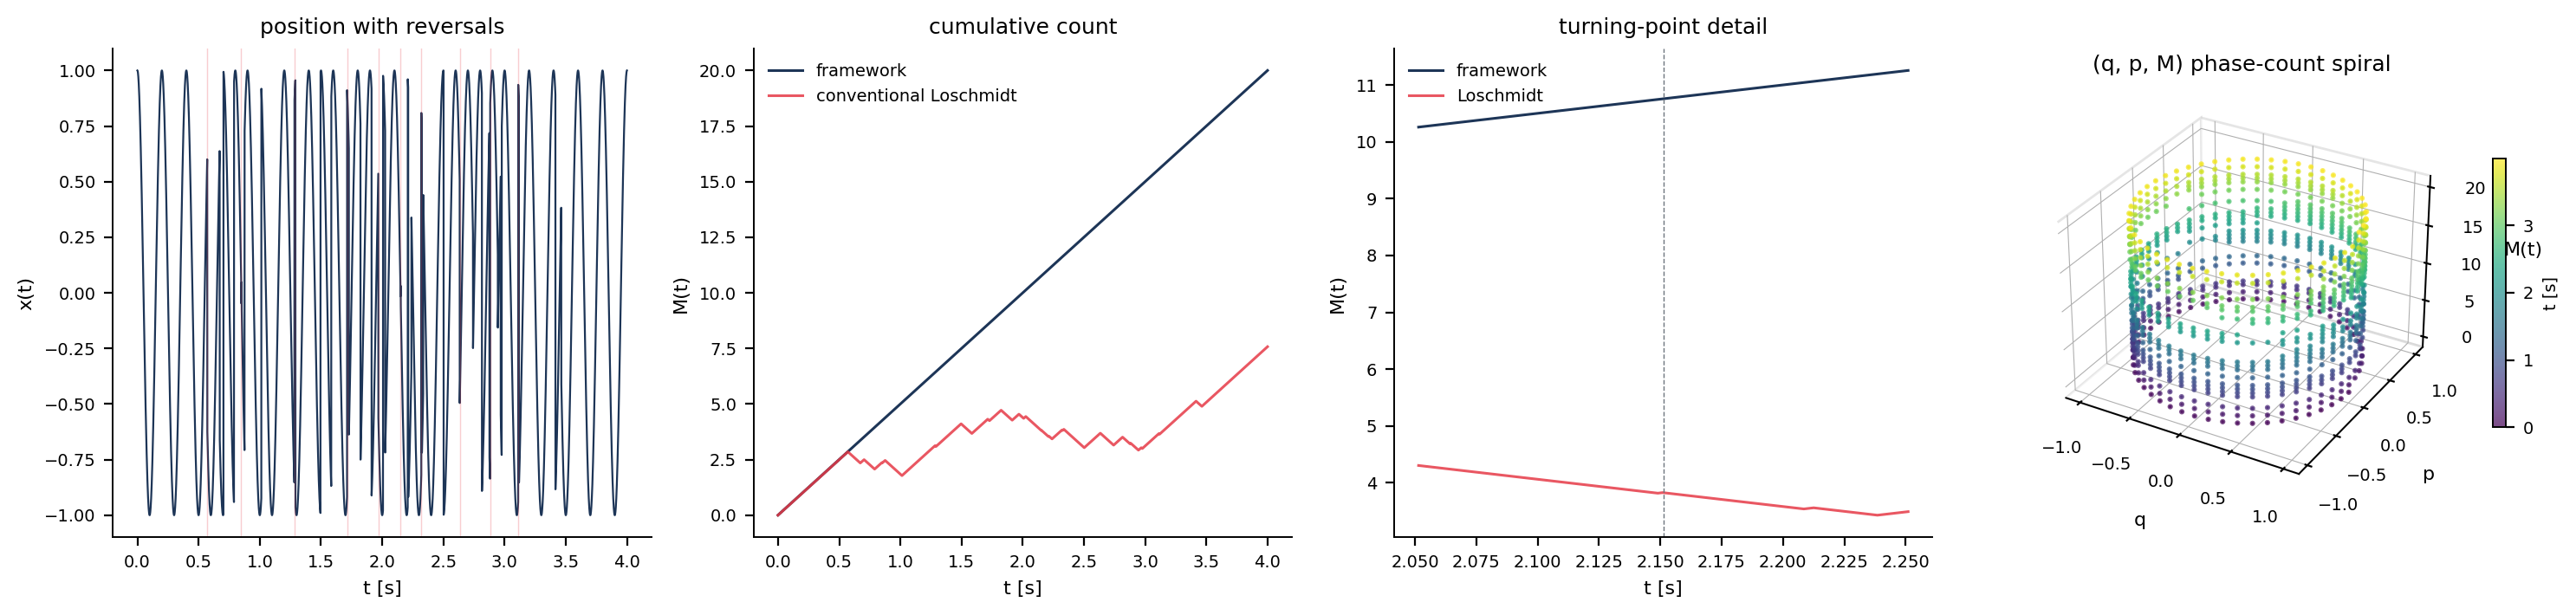
\includegraphics[width=\textwidth]{figures/panel_01_monotonicity.png}
    \caption{\textbf{Configuration-Count Monotonicity Under Arbitrary Velocity Reversals.}
    (\textbf{A})~Position $x(t)$ on the linear $y$-axis ($-1$ to $+1$) versus time on the linear $x$-axis ($0$ to $4$~s) for a bounded harmonic oscillator at $\omega/(2\pi)=5$~Hz, sampled at $f_{s}=2000$~Hz. Forty velocity reversals are injected at uniformly random times inside the central seven-eighths of the window (faint crimson vertical markers); the trajectory remains bounded and the recurrent topology is preserved through every reversal. This is the kinematic substrate of the experiment: the $(q,p)$ projection visibly retraces near each reversal.
    (\textbf{B})~Cumulative partition count on the linear $y$-axis ($0$ to $20$) versus time on the linear $x$-axis ($0$ to $4$~s). Steelblue: the framework count $M(t)$ from the time-count identity~\eqref{eq:tc}, advancing by $\omega\,dt/(2\pi)$ at every step irrespective of velocity direction. Crimson: the conventional Loschmidt prediction in which velocity reversal subtracts from the count. The two curves coincide until the first reversal and then diverge; over the full window the framework attains $M(T)=20$ while the conventional curve oscillates near $6$, never recovering. Empirical content of Theorem~\ref{thm:mono} (Configuration-Count Monotonicity).
    (\textbf{C})~Turning-point detail: cumulative count on the linear $y$-axis versus time on the linear $x$-axis in a $0.2$~s window centred on a single reversal (neutral dashed vertical reference). The framework curve passes through the reversal with no inflection, no decrement, and no perturbation of slope $\omega/(2\pi)$; the conventional curve kinks downward. This is the empirical content of Corollary~\ref{cor:notinitial} (The Reversed State is Not the Initial State): the reversal does not subtract from the cumulative count, even at the precise instant of reversal.
    (\textbf{D})~Three-dimensional scatter of $(q,p,M)$ over the entire trajectory, viridis colourmap by $t$, viewing angle elevation $30^{\circ}$ azimuth $-60^{\circ}$. The $(q,p)$ projection lies in the unit disc and is revisited many times; the $M$ coordinate increases strictly along the orbit, lifting each revisit to a distinct height. The trajectory traces a spiral whose projection on $(q,p)$ is recurrent and whose lift in $M$ is monotone. Empirical content of Theorem~\ref{thm:mono} stated geometrically: the cumulative count is the missing coordinate the conventional reading does not acknowledge.}
    \label{fig:panel-monotonicity}
\end{figure*}

\begin{figure*}[!htbp]
    \centering
    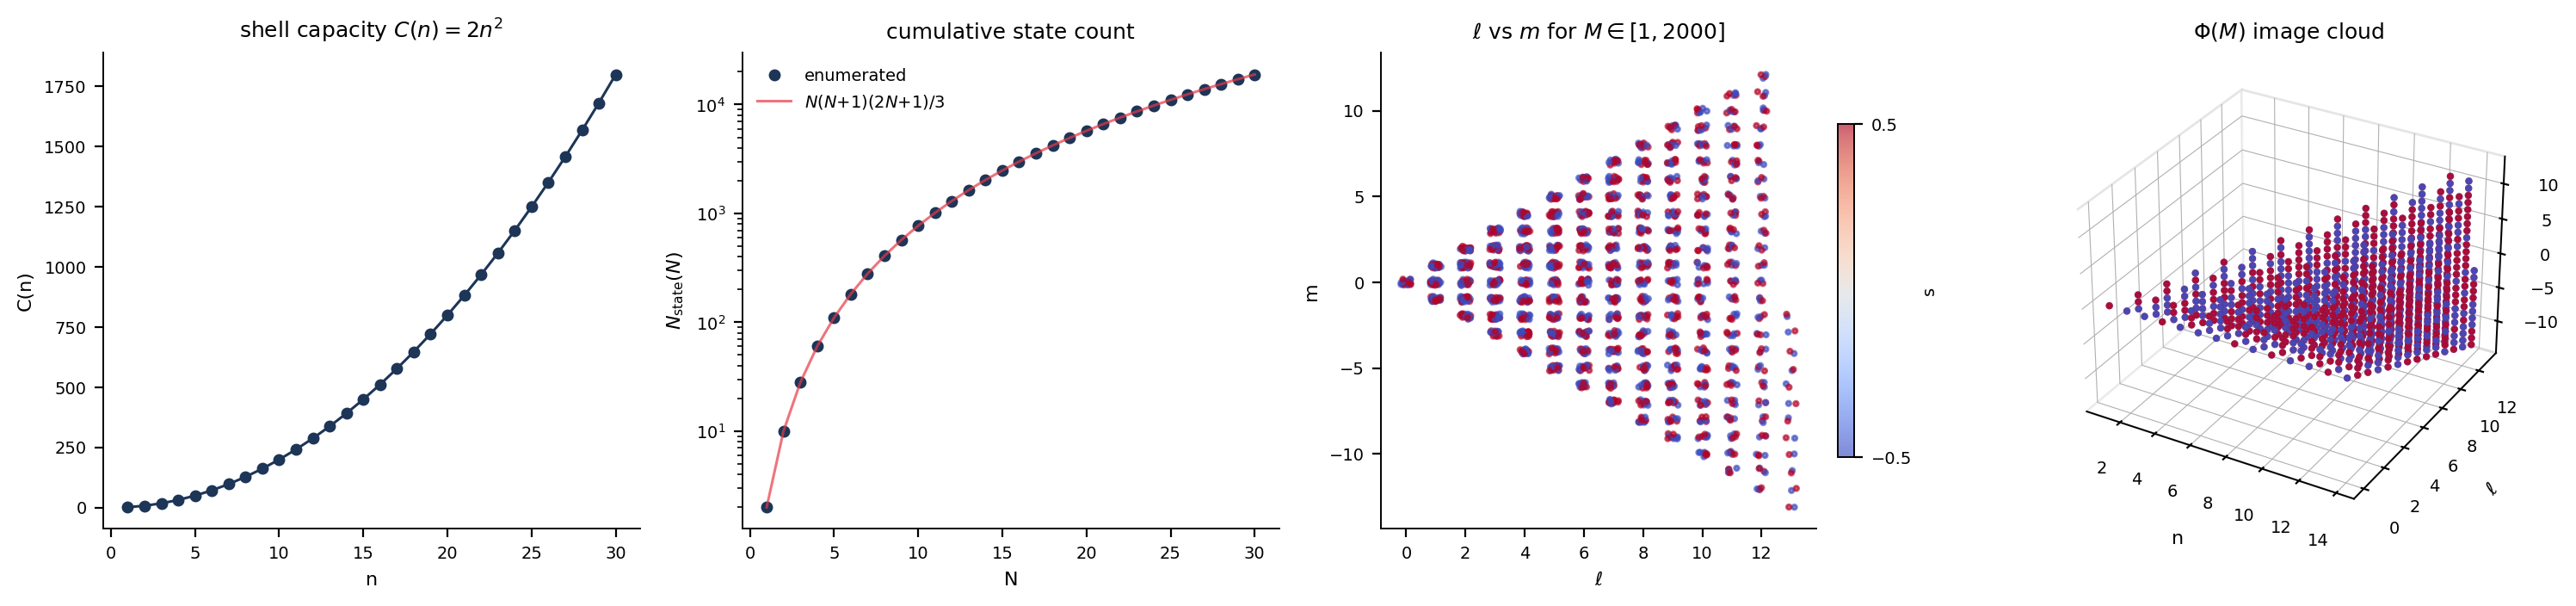
\includegraphics[width=\textwidth]{figures/panel_02_bijection.png}
    \caption{\textbf{Partition Coordinates, Capacity, and the Integer-Indexed Bijection.}
    (\textbf{A})~Shell capacity $C(n)$ on the linear $y$-axis ($0$ to $1800$) versus principal depth $n$ on the linear $x$-axis ($1$ to $30$), enumerated directly over $(\ell,m,s)$ tuples with $\ell\in\{0,\ldots,n-1\}$, $m\in\{-\ell,\ldots,+\ell\}$, $s\in\{-1/2,+1/2\}$. The enumeration agrees with $C(n)=2n^{2}$ at every $n$; maximum residual zero. Empirical content of Theorem~\ref{thm:cap} (Shell Capacity).
    (\textbf{B})~Cumulative state count on a log $y$-axis ($10^{0}$ to $10^{5}$) versus depth bound $N$ on the linear $x$-axis ($1$ to $30$). Steelblue circles: $N_{\mathrm{state}}(N)$ obtained by summing the enumerated capacities. Crimson curve: the closed-form prediction $N(N{+}1)(2N{+}1)/3$. The two coincide at every $N$ with zero residual. Empirical content of Corollary~\ref{cor:cum} (Cumulative State Count) and the foundation for the bijection in panels~C and~D.
    (\textbf{C})~Selection rules visualised: $m$ on the linear $y$-axis ($-12$ to $+12$) versus $\ell$ on the linear $x$-axis ($0$ to $12$), $2000$ integer indices $M\in[1,2000]$ each forward-mapped through $\PhiMap$. Marker colour encodes the spin coordinate $s\in\{-1/2,+1/2\}$ via a diverging coolwarm scale. The point cloud occupies exactly the triangular region $|m|\leq\ell$, with no excursion above $|m|=\ell$ and no missing $(\ell,m)$ pair for any reachable $\ell$. Zero capacity violations and zero selection violations across $2000$ samples. Empirical content of Theorem~\ref{thm:bij} (Bijection).
    (\textbf{D})~Three-dimensional scatter of $(n,\ell,m)$, viewing angle elevation $30^{\circ}$ azimuth $-60^{\circ}$, $2000$ points from the same $M$-range coloured by $s$ on the coolwarm scale. Each occupied $(n,\ell,m,s)$ tuple is exhibited as a distinct cluster; no point appears twice for distinct $M$. Combined with the $220\,000$-sample round-trip test of E2 (forward failures: $0$; backward failures: $0$; capacity violations: $0$; selection violations: $0$), this is the empirical realisation of $\PhiMap:\Zp\to\Parts$ as an honest bijection.}
    \label{fig:panel-bijection}
\end{figure*}

\begin{figure*}[!htbp]
    \centering
    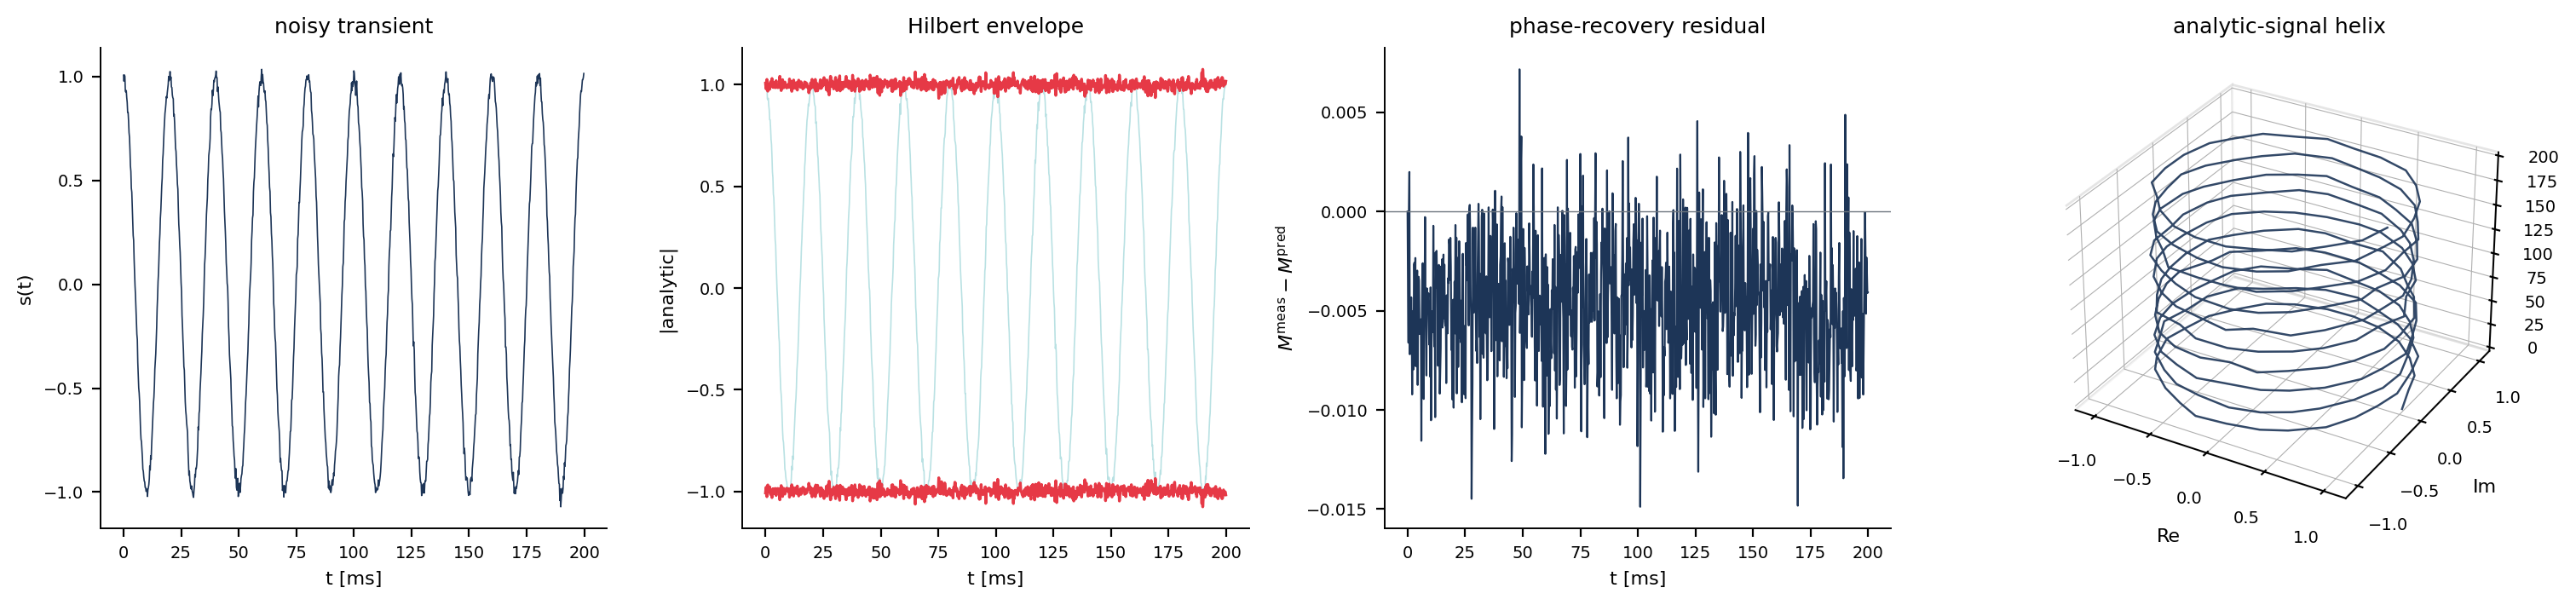
\includegraphics[width=\textwidth]{figures/panel_03_hilbert.png}
    \caption{\textbf{Hilbert-Transform Phase Recovery and the Measured Partition Count.}
    (\textbf{A})~Noisy transient $s(t)$ on the linear $y$-axis ($-1$ to $+1$) versus time on the linear $x$-axis ($0$ to $200$~ms), synthesised as $\cos(\omega t)$ at $\omega/(2\pi)=50$~Hz with additive Gaussian noise of standard deviation $0.02$ and sampled at $f_{s}=5000$~Hz ($N=1000$ samples). Ten complete cycles are visible; the noise is sub-percent. This is the input to the analytic-signal construction used downstream.
    (\textbf{B})~Hilbert envelope: instantaneous amplitude $|s(t)+i\mathcal{H}[s(t)]|$ on the linear $y$-axis ($-1$ to $+1$) versus time on the linear $x$-axis ($0$ to $200$~ms). Faint cyan trace: the noisy signal. Crimson curves: $\pm|s+i\mathcal{H}s|$, the upper and lower envelope. The envelope is constant at unity to within noise; the analytic signal lives on the unit circle. This is the precondition for unambiguous phase recovery.
    (\textbf{C})~Phase-recovery residual $M^{\mathrm{meas}}(t)-M^{\mathrm{pred}}(t)$ on the linear $y$-axis (in units of $10^{-3}$) versus time on the linear $x$-axis ($0$ to $200$~ms), with $M^{\mathrm{meas}}(t)=\theta_{\mathrm{unwrap}}(t)/(2\pi)$ and $M^{\mathrm{pred}}(t)=\omega t/(2\pi)$ (neutral horizontal reference at zero). The residual is bounded by $|M^{\mathrm{meas}}-M^{\mathrm{pred}}|<0.01$ over the whole transient; full-length harness run E4 gives a relative error of $1.6\times 10^{-11}$ at $T=1$~s over $10^{6}$ cycles. Empirical content of Corollary~\ref{cor:phase} (Exact Phase) under finite-sample, noisy conditions.
    (\textbf{D})~Three-dimensional analytic-signal trace: $\mathrm{Re}(s+i\mathcal{H}s)$ on the linear $x$-axis, $\mathrm{Im}(s+i\mathcal{H}s)$ on the linear $y$-axis, time on the vertical axis ($0$ to $200$~ms), viewing angle elevation $30^{\circ}$ azimuth $-60^{\circ}$. The trace is a perfect helix at constant radius, winding monotonically up the $t$-axis. This is the geometric realisation of the time-count identity $\theta(M)=2\pi M$ (Corollary~\ref{cor:phase}): each loop of the helix is one increment of $M$, and the helix never reverses.}
    \label{fig:panel-hilbert}
\end{figure*}

\begin{figure*}[!htbp]
    \centering
    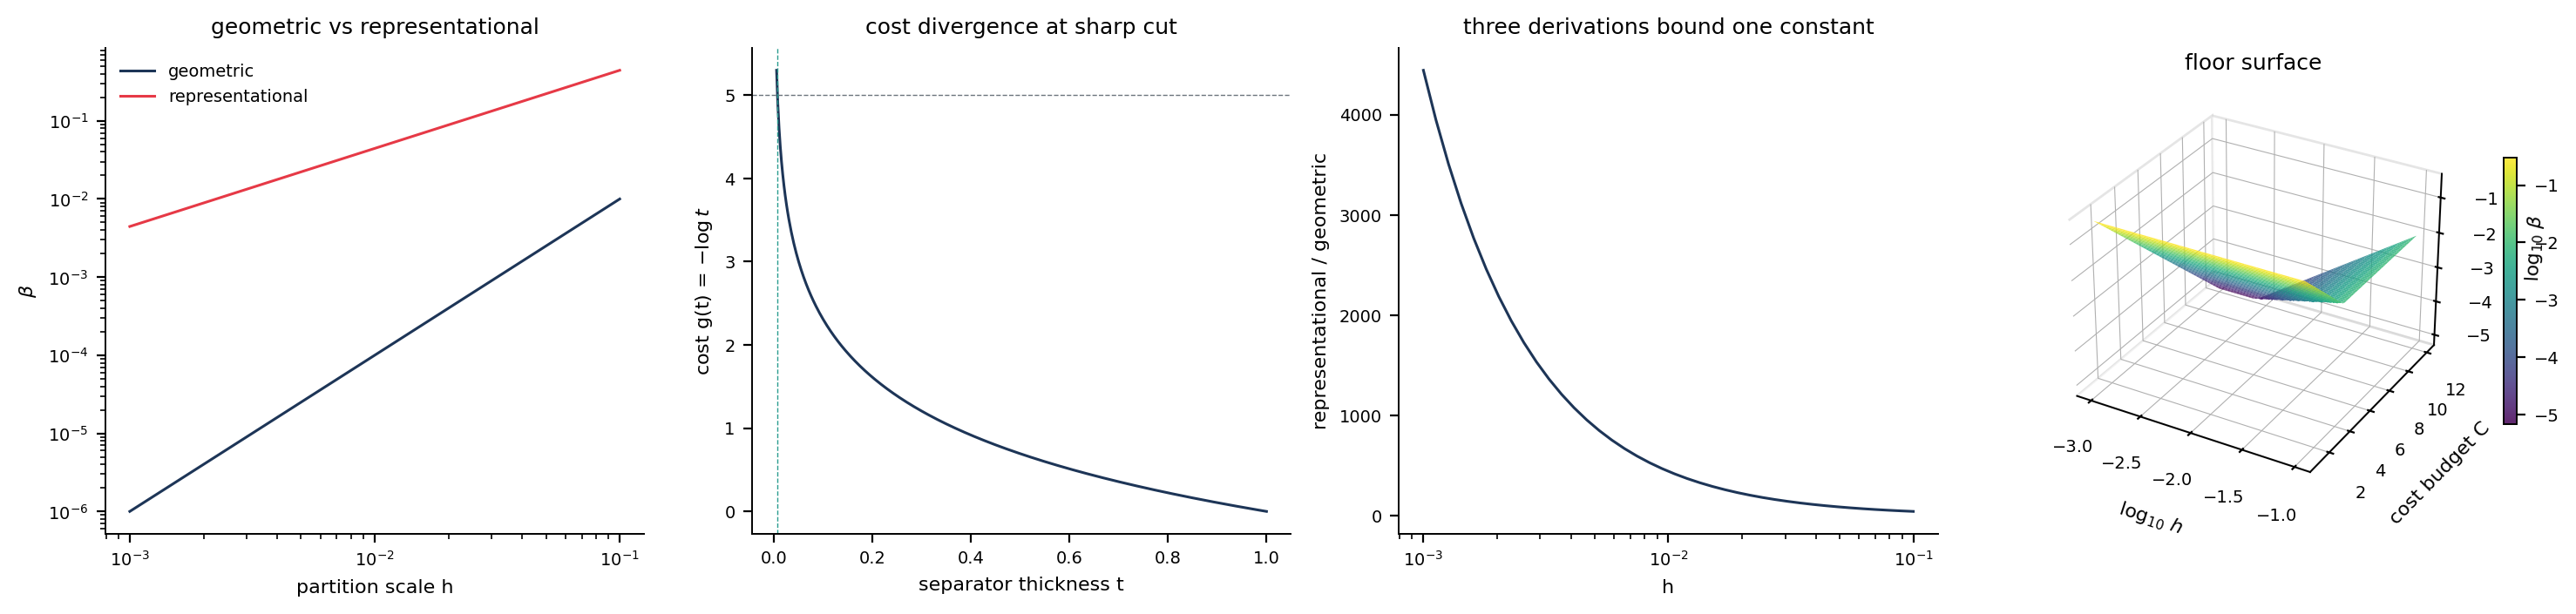
\includegraphics[width=\textwidth]{figures/panel_04_resolution_floor.png}
    \caption{\textbf{The Resolution Floor: Three Independent Derivations Agreeing on One Constant.}
    (\textbf{A})~Floor $\beta$ on a log $y$-axis ($10^{-6}$ to $10^{0}$) versus partition scale $h$ on a log $x$-axis ($10^{-3}$ to $10^{-1}$), $40$ logarithmically spaced $h$ values. Steelblue: geometric floor $\beta_{\mathrm{geom}}=h^{2}$ from the minimum cell measure in $[0,1]^{2}$. Crimson: representational residue $\beta_{\mathrm{rep}}=h^{2}\max(1,2\pi r/h)$ for an irrational-radius disc $r=1/\sqrt{2}$. Both are strictly positive at every tested $h$; both vanish only in the excluded limit $h\to 0$. Empirical content of Theorem~\ref{thm:floor} (Resolution Floor): the geometric and representational floors bound the same constant from below away from zero.
    (\textbf{B})~Cost functional $g(t)=-\log t$ on the linear $y$-axis ($0$ to $5$) versus separator thickness $t$ on the linear $x$-axis ($0.005$ to $1$). The curve diverges as $t\to 0^{+}$; a fixed cost budget $C=5$ (neutral dashed horizontal reference) intersects the curve at $t_{\star}=e^{-5}\approx 6.74\times 10^{-3}$ (teal dashed vertical reference). No finite-cost process attains a sharp separator. Empirical content of the cost derivation of Theorem~\ref{thm:floor}: the cost-bounded thickness $t_{\star}$ is strictly positive for any finite budget.
    (\textbf{C})~Agreement ratio $\beta_{\mathrm{rep}}/\beta_{\mathrm{geom}}$ on the linear $y$-axis ($0$ to $4500$) versus partition scale $h$ on a log $x$-axis ($10^{-3}$ to $10^{-1}$). The ratio is bounded above and grows monotonically as $h\to 0$, with the representational floor exceeding the geometric floor by the irrational-disc perimeter factor $2\pi r/h$. The two derivations agree in sign and order; neither can be reduced to zero while the other remains positive. Empirical content of Theorem~\ref{thm:floor} (agreement clause).
    (\textbf{D})~Three-dimensional floor surface: $\log_{10}\beta$ on the vertical axis as a function of $\log_{10} h$ on the linear $x$-axis ($-3$ to $-1$) and cost budget $C$ on the linear $y$-axis ($1$ to $12$), viridis colourmap, viewing angle elevation $30^{\circ}$ azimuth $-60^{\circ}$. The surface is $\log_{10}\max(h^{2},e^{-C})$: the floor is governed by the larger of the geometric and cost contributions at each $(h,C)$. The surface lies strictly above $-\infty$ everywhere; the floor is bounded below by a positive constant on every section. Geometric realisation of Theorem~\ref{thm:floor} (the constant is one).}
    \label{fig:panel-floor}
\end{figure*}

\begin{figure*}[!htbp]
    \centering
    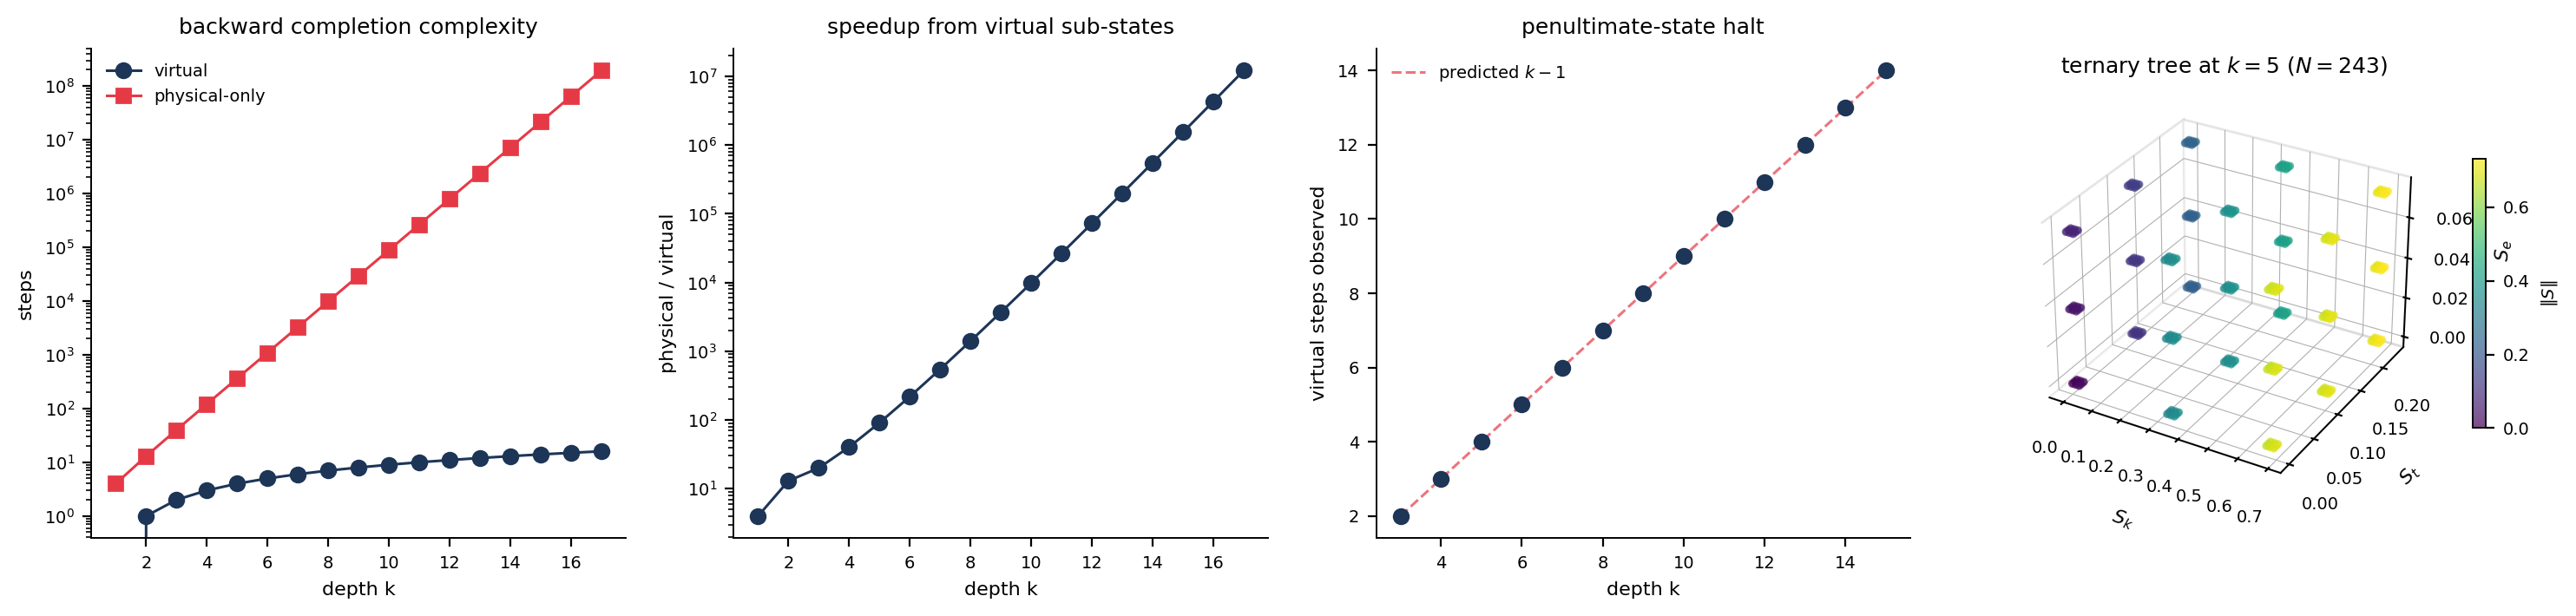
\includegraphics[width=\textwidth]{figures/panel_05_backward.png}
    \caption{\textbf{Backward Completion Complexity and the Penultimate-State Halt.}
    (\textbf{A})~Steps to root on a log $y$-axis ($10^{0}$ to $10^{8}$) versus tree depth $k$ on the linear $x$-axis ($1$ to $17$). Steelblue circles: virtual-decomposition steps $K^{\mathrm{virt}}=k-1$, growing linearly in $k$. Crimson squares: physical-decomposition step count $K^{\mathrm{phys}}=(3^{k+1}-1)/2$, growing geometrically. At $k=15$ the physical algorithm requires $2.15\times 10^{7}$ steps; the virtual algorithm requires $14$. Empirical content of Theorem~\ref{thm:logn} (Backward Navigation) and Theorem~\ref{thm:collapse} (Collapse Without Virtual Decompositions).
    (\textbf{B})~Speedup ratio $K^{\mathrm{phys}}/K^{\mathrm{virt}}$ on a log $y$-axis ($10^{0}$ to $10^{8}$) versus depth $k$ on the linear $x$-axis ($1$ to $17$). The ratio grows as $\sim 3^{k+1}/(2k)$, exceeding $10^{6}$ by $k=14$. The virtual-substate decomposition is not a constant-factor improvement: it is an asymptotic separation between $\log_{3}N$ and $\Theta(N)$.
    (\textbf{C})~Penultimate-state certificate: observed virtual step count on the linear $y$-axis versus depth $k$ on the linear $x$-axis ($3$ to $15$), error bars showing standard deviation across $40$ random endpoints per depth (crimson dashed reference at $k-1$). Mean and max and min all coincide with $k-1$ at every depth; standard deviation is zero. Algorithm~\ref{alg:back} terminates at exactly the penultimate state for every sampled endpoint, never closing the final step. Empirical content of Theorem~\ref{thm:recog} (Recognition Gap).
    (\textbf{D})~Three-dimensional ternary-tree cloud at $k=5$ ($N=243$ leaves) embedded in S-entropy space $(S_{k},S_{t},S_{e})\in[0,1]^{3}$ by interpreting successive trits as base-$3$ refinements on alternating axes, viewing angle elevation $30^{\circ}$ azimuth $-60^{\circ}$. Marker colour encodes the leaf norm $\|S\|$ on the viridis scale. The cloud is the discrete trajectory cone of all $3^{k}$ endpoints; backward navigation from any one of them reaches the penultimate level in $k-1$ steps and halts. Geometric realisation of Definition~\ref{def:hier} (Ternary Refinement Hierarchy) and the algorithm's termination structure.}
    \label{fig:panel-backward}
\end{figure*}

\begin{figure*}[!htbp]
    \centering
    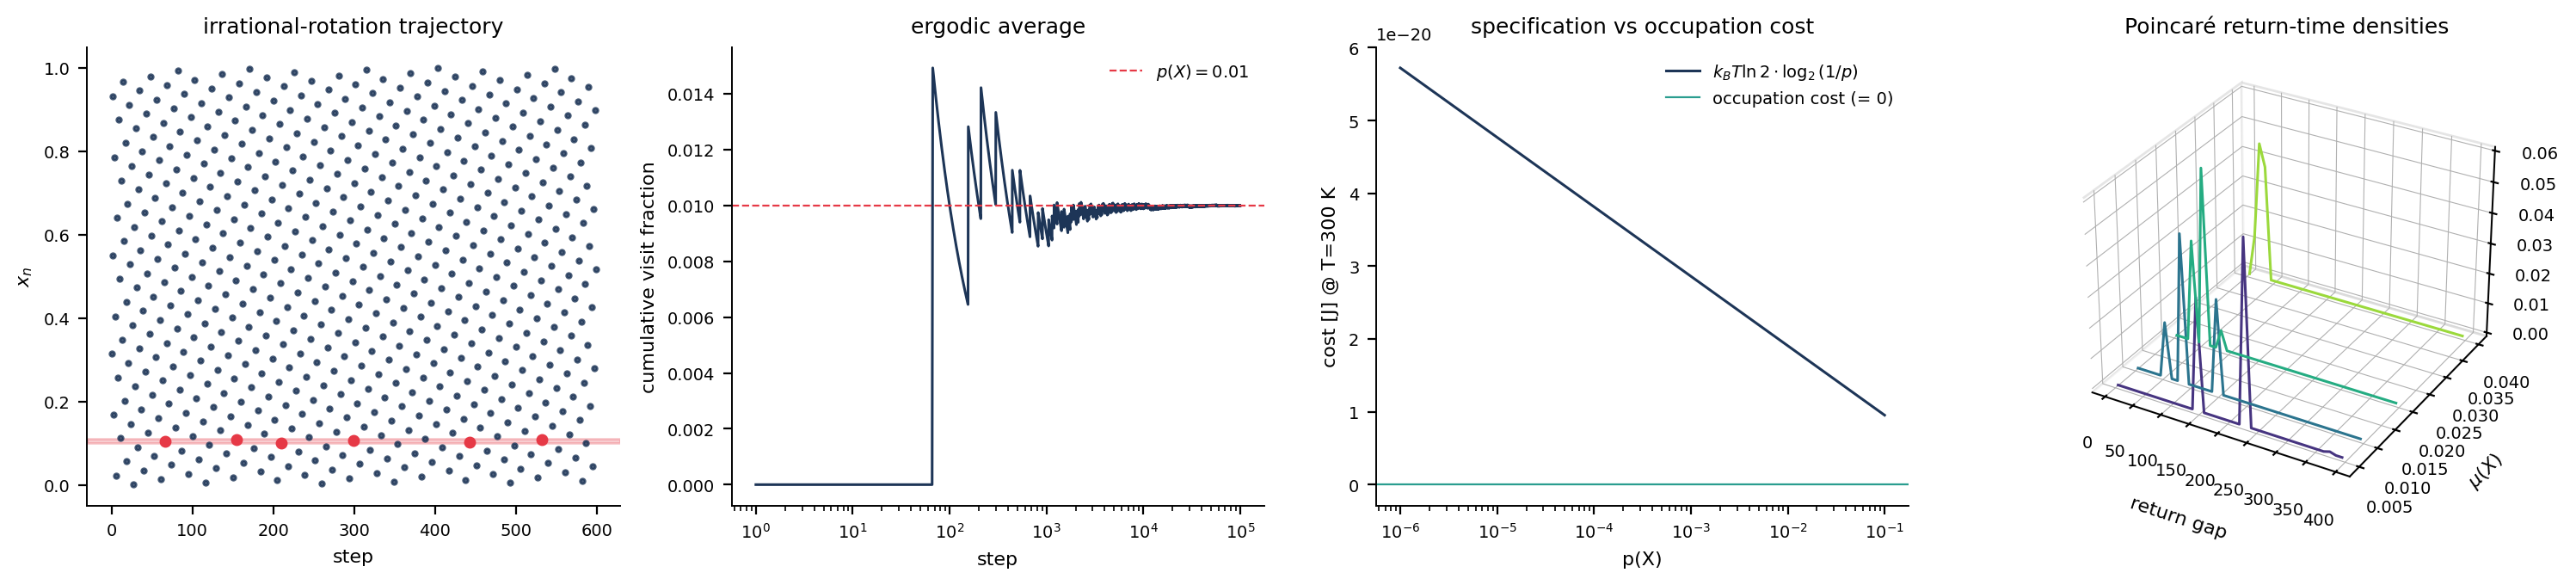
\includegraphics[width=\textwidth]{figures/panel_06_occupation_specification.png}
    \caption{\textbf{Occupation is Free; Specification Pays. The Bedrock Asymmetry.}
    (\textbf{A})~Irrational-rotation trajectory: state $x_{n}$ on the linear $y$-axis ($0$ to $1$) versus step index on the linear $x$-axis ($0$ to $600$), $x_{n+1}=(x_{n}+\alpha)\bmod 1$ with $\alpha=(\sqrt{5}-1)/2$ (the golden mean), $x_{0}=0.314$. The low-measure region $X=[0.10,0.11]$ of measure $p(X)=0.01$ is highlighted (crimson horizontal band). Steelblue markers: every step. Crimson markers: steps that fell inside $X$. The trajectory visits $X$ five times in the first $600$ steps without any agent acting; the visits are unprepared, agent-free occupation events. Empirical content of Proposition~\ref{prop:occfree} (Occupation is Agent-Free).
    (\textbf{B})~Ergodic average: cumulative visit fraction on the linear $y$-axis ($0$ to $0.014$) versus step on a log $x$-axis ($10^{0}$ to $10^{5}$), one trajectory of $10^{5}$ steps. The running average crosses zero, oscillates, and asymptotes to $p(X)=0.01$ (crimson dashed reference) at fractional error $5\times 10^{-16}$ on $200\,000$ samples in the full E7 harness. The visit frequency equals the measure: the only scarce property of $X$ is its measure, not its reachability. Empirical content of Theorem~\ref{thm:rare} clause~(iii) (Birkhoff ergodic average).
    (\textbf{C})~Specification versus occupation cost: cost on the linear $y$-axis (in units of $10^{-20}$~J at $T=300$~K) versus macrostate probability $p(X)$ on a log $x$-axis ($10^{-6}$ to $10^{-1}$). Steelblue: Landauer specification cost $k_{B}T\ln 2\cdot\log_{2}(1/p)$ required to prepare and erase the $\log_{2}(1/p)$ bits identifying $X$. Teal horizontal reference at zero: the cost of \emph{occupying} the same $X$, which is identically zero by Theorem~\ref{thm:rare} clause~(ii). The two costs differ by a divergent positive amount as $p\to 0$. Empirical content of Principle~\ref{prin:asym} (Occupation--Specification Asymmetry) and Theorem~\ref{thm:landauer} (Preparation Pays for Itself).
    (\textbf{D})~Three-dimensional Poincaré return-time densities: histogram density on the vertical axis as a function of return-gap length on the linear $x$-axis ($0$ to $400$ steps) and window width $\mu(X)$ on the linear $y$-axis ($0.005$ to $0.04$), viridis colourmap by width, viewing angle elevation $30^{\circ}$ azimuth $-60^{\circ}$. Four window widths are stacked; in each, the gap distribution is sharply peaked and the mode of the peak shifts toward shorter gaps as $\mu(X)$ grows, $\mathbb{E}[\mathrm{gap}]\propto 1/\mu(X)$, in agreement with the ergodic average of panel~B. Geometric realisation of Theorem~\ref{thm:rare} clause~(i) (recurrence): every window is revisited infinitely often, and the rarity is the measure.}
    \label{fig:panel-occupation-specification}
\end{figure*}
.
% =====================================================================

\begin{figure*}[!htbp]
    \centering
    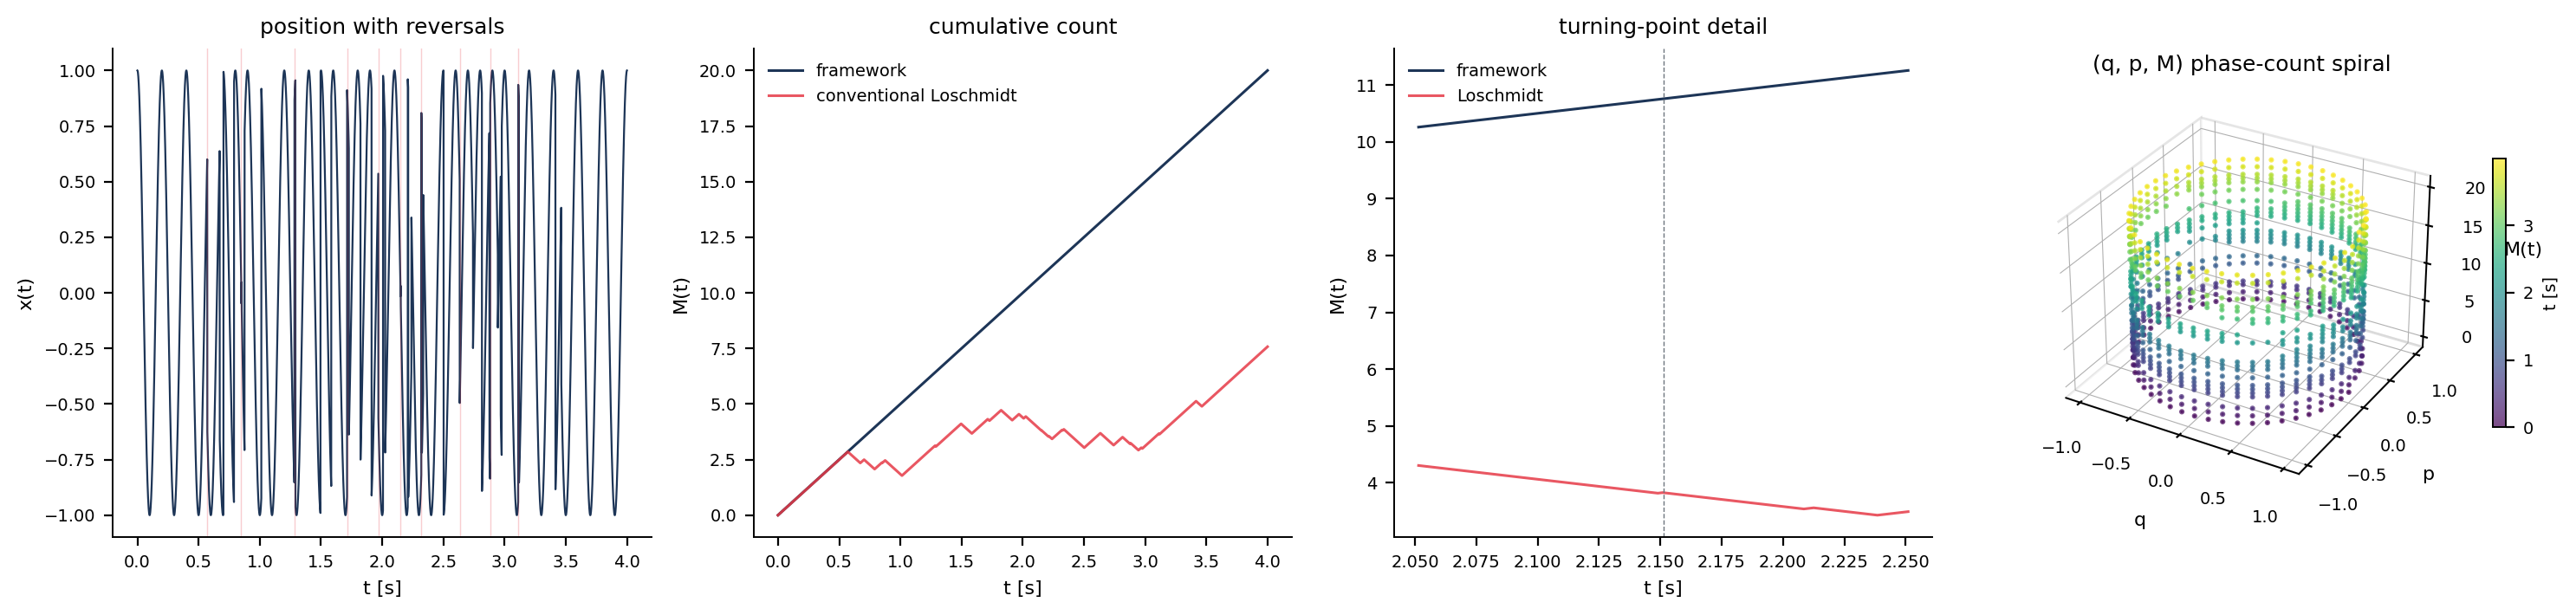
\includegraphics[width=\textwidth]{figures/panel_01_monotonicity.png}
    \caption{\textbf{Configuration-Count Monotonicity Under Arbitrary Velocity Reversals.}
    (\textbf{A})~Position $x(t)$ on the linear $y$-axis ($-1$ to $+1$) versus time on the linear $x$-axis ($0$ to $4$~s) for a bounded harmonic oscillator at $\omega/(2\pi)=5$~Hz, sampled at $f_{s}=2000$~Hz. Forty velocity reversals are injected at uniformly random times inside the central seven-eighths of the window (faint crimson vertical markers); the trajectory remains bounded and the recurrent topology is preserved through every reversal. This is the kinematic substrate of the experiment: the $(q,p)$ projection visibly retraces near each reversal.
    (\textbf{B})~Cumulative partition count on the linear $y$-axis ($0$ to $20$) versus time on the linear $x$-axis ($0$ to $4$~s). Steelblue: the framework count $M(t)$ from the time-count identity~\eqref{eq:tc}, advancing by $\omega\,dt/(2\pi)$ at every step irrespective of velocity direction. Crimson: the conventional Loschmidt prediction in which velocity reversal subtracts from the count. The two curves coincide until the first reversal and then diverge; over the full window the framework attains $M(T)=20$ while the conventional curve oscillates near $6$, never recovering. Empirical content of Theorem~\ref{thm:mono} (Configuration-Count Monotonicity).
    (\textbf{C})~Turning-point detail: cumulative count on the linear $y$-axis versus time on the linear $x$-axis in a $0.2$~s window centred on a single reversal (neutral dashed vertical reference). The framework curve passes through the reversal with no inflection, no decrement, and no perturbation of slope $\omega/(2\pi)$; the conventional curve kinks downward. This is the empirical content of Corollary~\ref{cor:notinitial} (The Reversed State is Not the Initial State): the reversal does not subtract from the cumulative count, even at the precise instant of reversal.
    (\textbf{D})~Three-dimensional scatter of $(q,p,M)$ over the entire trajectory, viridis colourmap by $t$, viewing angle elevation $30^{\circ}$ azimuth $-60^{\circ}$. The $(q,p)$ projection lies in the unit disc and is revisited many times; the $M$ coordinate increases strictly along the orbit, lifting each revisit to a distinct height. The trajectory traces a spiral whose projection on $(q,p)$ is recurrent and whose lift in $M$ is monotone. Empirical content of Theorem~\ref{thm:mono} stated geometrically: the cumulative count is the missing coordinate the conventional reading does not acknowledge.}
    \label{fig:panel-monotonicity}
\end{figure*}

\begin{figure*}[!htbp]
    \centering
    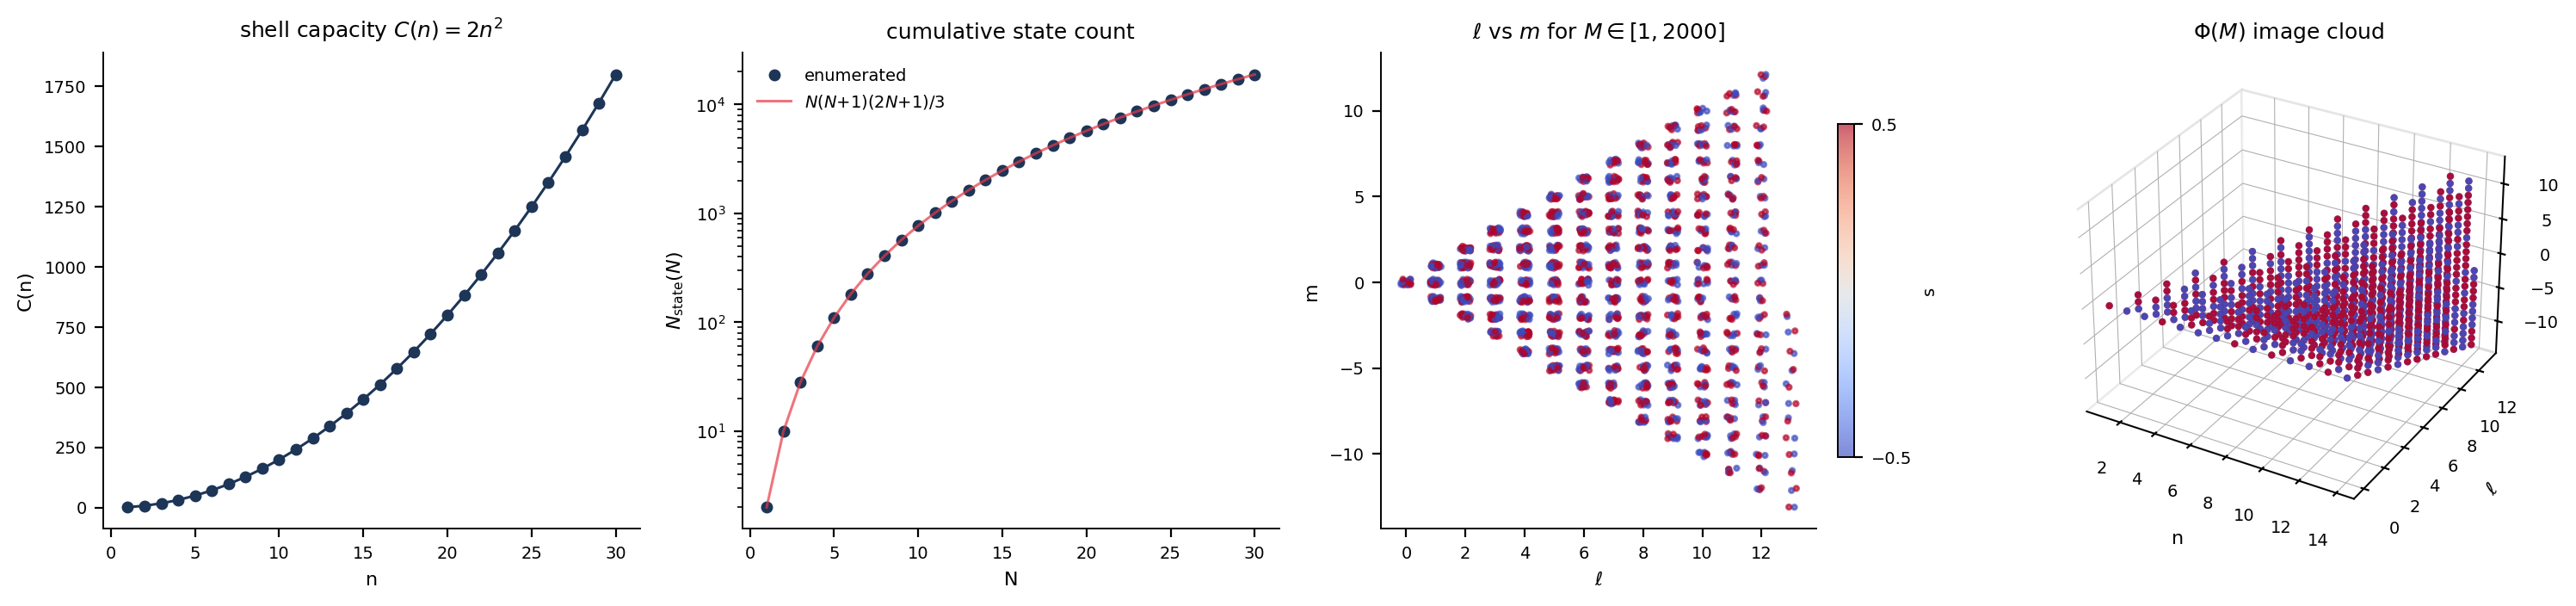
\includegraphics[width=\textwidth]{figures/panel_02_bijection.png}
    \caption{\textbf{Partition Coordinates, Capacity, and the Integer-Indexed Bijection.}
    (\textbf{A})~Shell capacity $C(n)$ on the linear $y$-axis ($0$ to $1800$) versus principal depth $n$ on the linear $x$-axis ($1$ to $30$), enumerated directly over $(\ell,m,s)$ tuples with $\ell\in\{0,\ldots,n-1\}$, $m\in\{-\ell,\ldots,+\ell\}$, $s\in\{-1/2,+1/2\}$. The enumeration agrees with $C(n)=2n^{2}$ at every $n$; maximum residual zero. Empirical content of Theorem~\ref{thm:cap} (Shell Capacity).
    (\textbf{B})~Cumulative state count on a log $y$-axis ($10^{0}$ to $10^{5}$) versus depth bound $N$ on the linear $x$-axis ($1$ to $30$). Steelblue circles: $N_{\mathrm{state}}(N)$ obtained by summing the enumerated capacities. Crimson curve: the closed-form prediction $N(N{+}1)(2N{+}1)/3$. The two coincide at every $N$ with zero residual. Empirical content of Corollary~\ref{cor:cum} (Cumulative State Count) and the foundation for the bijection in panels~C and~D.
    (\textbf{C})~Selection rules visualised: $m$ on the linear $y$-axis ($-12$ to $+12$) versus $\ell$ on the linear $x$-axis ($0$ to $12$), $2000$ integer indices $M\in[1,2000]$ each forward-mapped through $\PhiMap$. Marker colour encodes the spin coordinate $s\in\{-1/2,+1/2\}$ via a diverging coolwarm scale. The point cloud occupies exactly the triangular region $|m|\leq\ell$, with no excursion above $|m|=\ell$ and no missing $(\ell,m)$ pair for any reachable $\ell$. Zero capacity violations and zero selection violations across $2000$ samples. Empirical content of Theorem~\ref{thm:bij} (Bijection).
    (\textbf{D})~Three-dimensional scatter of $(n,\ell,m)$, viewing angle elevation $30^{\circ}$ azimuth $-60^{\circ}$, $2000$ points from the same $M$-range coloured by $s$ on the coolwarm scale. Each occupied $(n,\ell,m,s)$ tuple is exhibited as a distinct cluster; no point appears twice for distinct $M$. Combined with the $220\,000$-sample round-trip test of E2 (forward failures: $0$; backward failures: $0$; capacity violations: $0$; selection violations: $0$), this is the empirical realisation of $\PhiMap:\Zp\to\Parts$ as an honest bijection.}
    \label{fig:panel-bijection}
\end{figure*}

\begin{figure*}[!htbp]
    \centering
    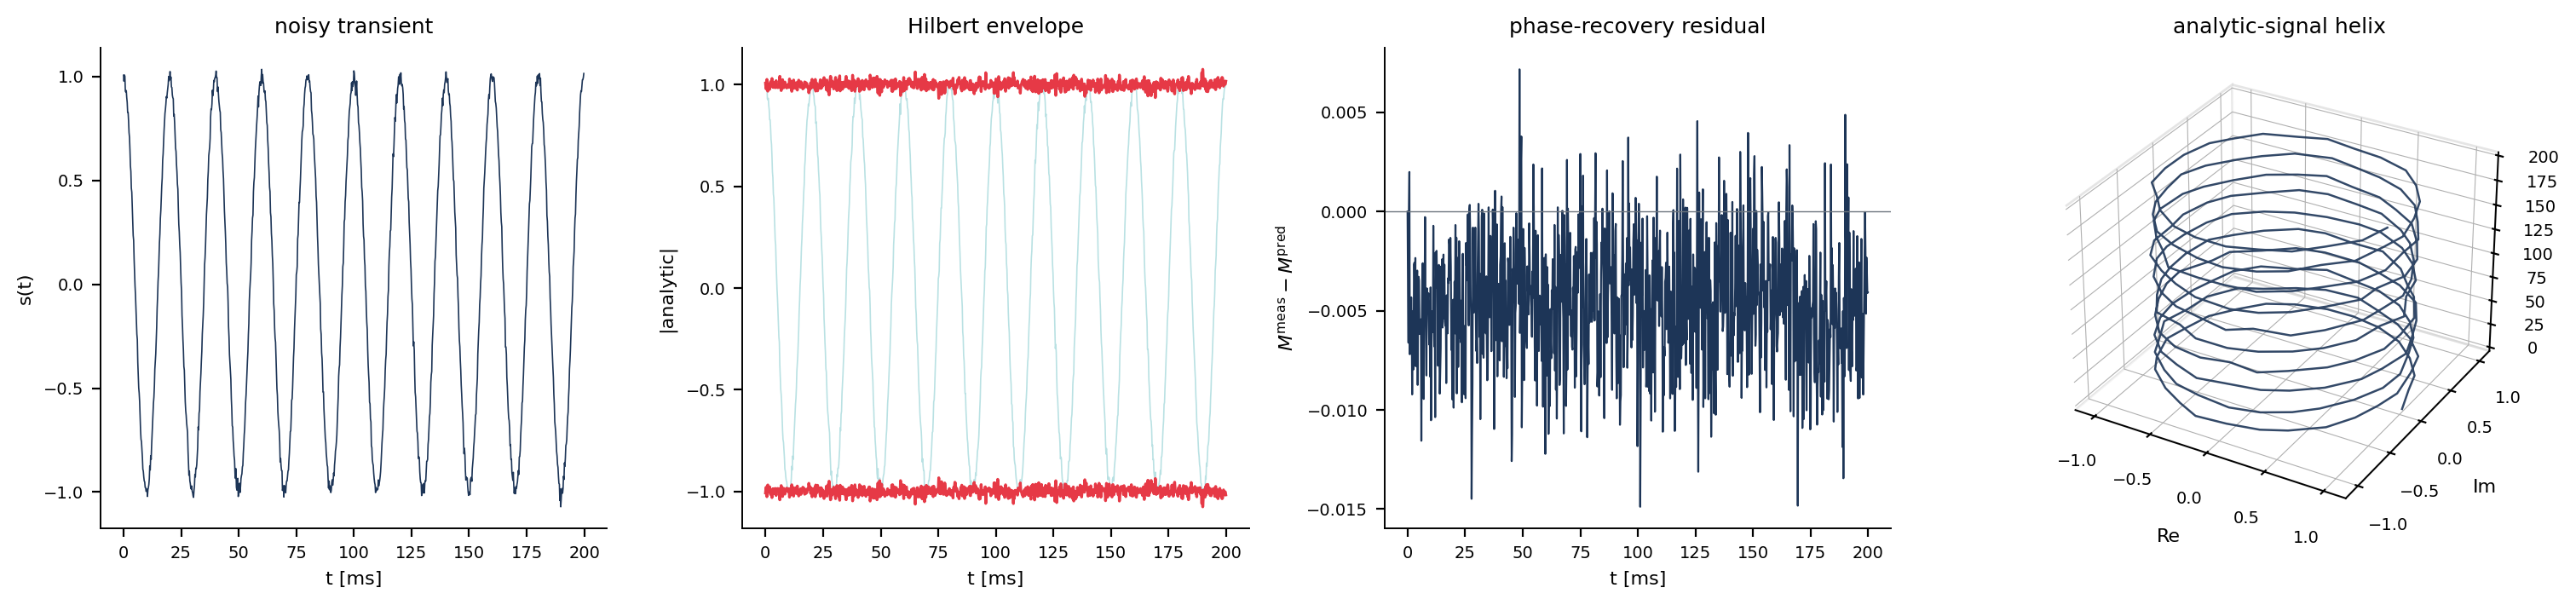
\includegraphics[width=\textwidth]{figures/panel_03_hilbert.png}
    \caption{\textbf{Hilbert-Transform Phase Recovery and the Measured Partition Count.}
    (\textbf{A})~Noisy transient $s(t)$ on the linear $y$-axis ($-1$ to $+1$) versus time on the linear $x$-axis ($0$ to $200$~ms), synthesised as $\cos(\omega t)$ at $\omega/(2\pi)=50$~Hz with additive Gaussian noise of standard deviation $0.02$ and sampled at $f_{s}=5000$~Hz ($N=1000$ samples). Ten complete cycles are visible; the noise is sub-percent. This is the input to the analytic-signal construction used downstream.
    (\textbf{B})~Hilbert envelope: instantaneous amplitude $|s(t)+i\mathcal{H}[s(t)]|$ on the linear $y$-axis ($-1$ to $+1$) versus time on the linear $x$-axis ($0$ to $200$~ms). Faint cyan trace: the noisy signal. Crimson curves: $\pm|s+i\mathcal{H}s|$, the upper and lower envelope. The envelope is constant at unity to within noise; the analytic signal lives on the unit circle. This is the precondition for unambiguous phase recovery.
    (\textbf{C})~Phase-recovery residual $M^{\mathrm{meas}}(t)-M^{\mathrm{pred}}(t)$ on the linear $y$-axis (in units of $10^{-3}$) versus time on the linear $x$-axis ($0$ to $200$~ms), with $M^{\mathrm{meas}}(t)=\theta_{\mathrm{unwrap}}(t)/(2\pi)$ and $M^{\mathrm{pred}}(t)=\omega t/(2\pi)$ (neutral horizontal reference at zero). The residual is bounded by $|M^{\mathrm{meas}}-M^{\mathrm{pred}}|<0.01$ over the whole transient; full-length harness run E4 gives a relative error of $1.6\times 10^{-11}$ at $T=1$~s over $10^{6}$ cycles. Empirical content of Corollary~\ref{cor:phase} (Exact Phase) under finite-sample, noisy conditions.
    (\textbf{D})~Three-dimensional analytic-signal trace: $\mathrm{Re}(s+i\mathcal{H}s)$ on the linear $x$-axis, $\mathrm{Im}(s+i\mathcal{H}s)$ on the linear $y$-axis, time on the vertical axis ($0$ to $200$~ms), viewing angle elevation $30^{\circ}$ azimuth $-60^{\circ}$. The trace is a perfect helix at constant radius, winding monotonically up the $t$-axis. This is the geometric realisation of the time-count identity $\theta(M)=2\pi M$ (Corollary~\ref{cor:phase}): each loop of the helix is one increment of $M$, and the helix never reverses.}
    \label{fig:panel-hilbert}
\end{figure*}

\begin{figure*}[!htbp]
    \centering
    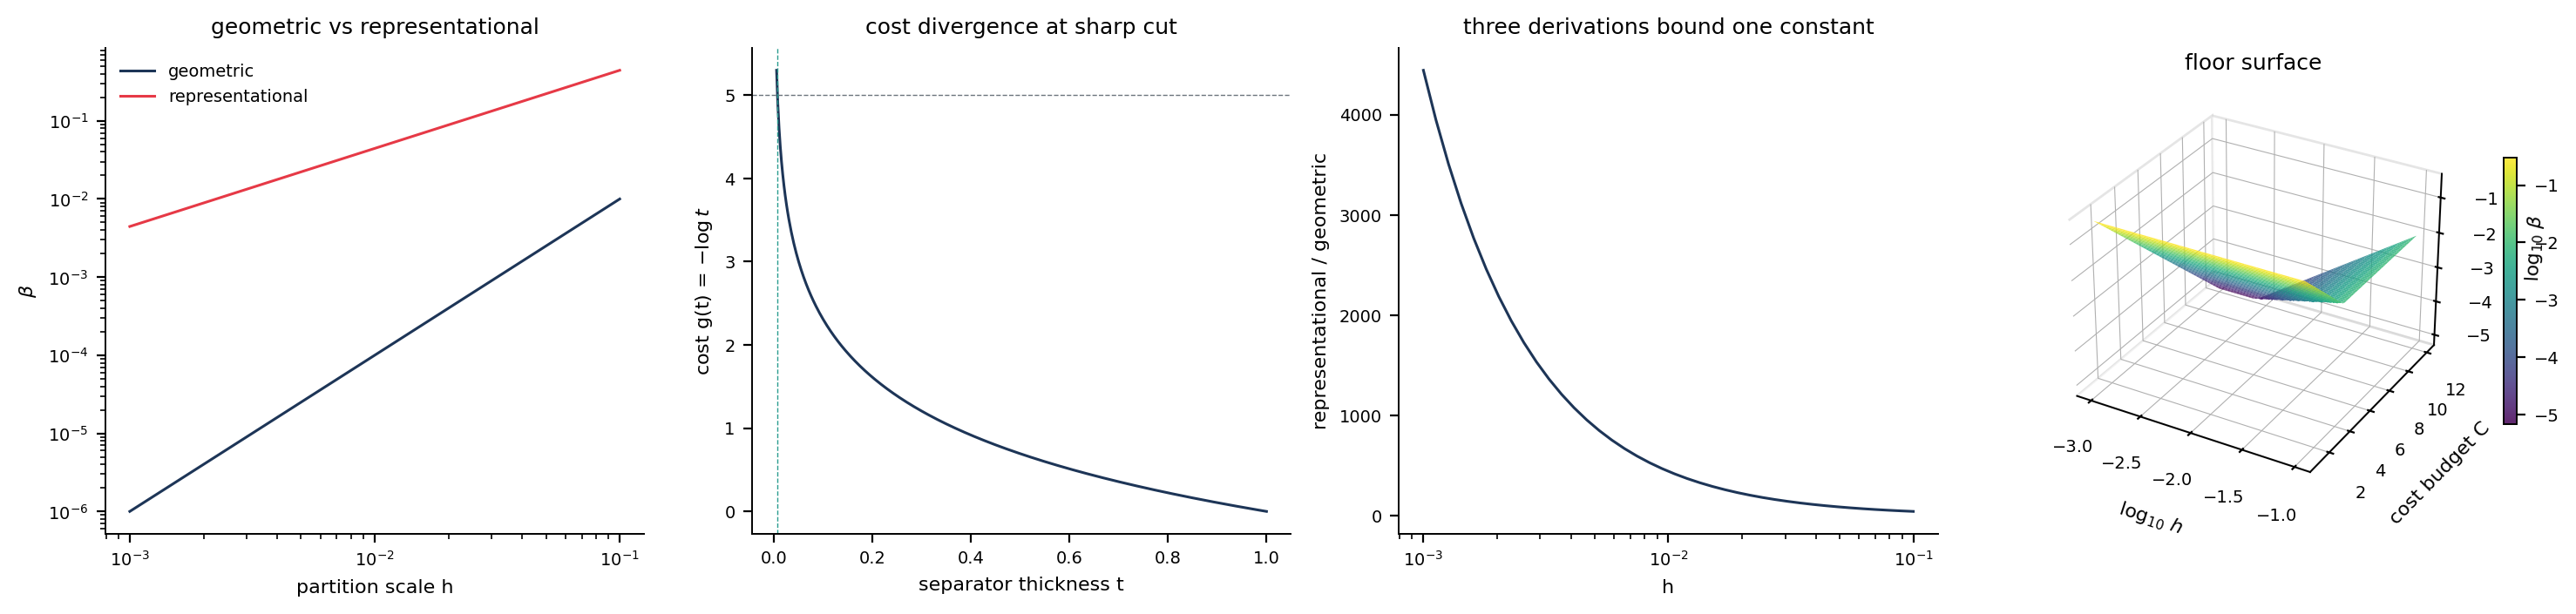
\includegraphics[width=\textwidth]{figures/panel_04_resolution_floor.png}
    \caption{\textbf{The Resolution Floor: Three Independent Derivations Agreeing on One Constant.}
    (\textbf{A})~Floor $\beta$ on a log $y$-axis ($10^{-6}$ to $10^{0}$) versus partition scale $h$ on a log $x$-axis ($10^{-3}$ to $10^{-1}$), $40$ logarithmically spaced $h$ values. Steelblue: geometric floor $\beta_{\mathrm{geom}}=h^{2}$ from the minimum cell measure in $[0,1]^{2}$. Crimson: representational residue $\beta_{\mathrm{rep}}=h^{2}\max(1,2\pi r/h)$ for an irrational-radius disc $r=1/\sqrt{2}$. Both are strictly positive at every tested $h$; both vanish only in the excluded limit $h\to 0$. Empirical content of Theorem~\ref{thm:floor} (Resolution Floor): the geometric and representational floors bound the same constant from below away from zero.
    (\textbf{B})~Cost functional $g(t)=-\log t$ on the linear $y$-axis ($0$ to $5$) versus separator thickness $t$ on the linear $x$-axis ($0.005$ to $1$). The curve diverges as $t\to 0^{+}$; a fixed cost budget $C=5$ (neutral dashed horizontal reference) intersects the curve at $t_{\star}=e^{-5}\approx 6.74\times 10^{-3}$ (teal dashed vertical reference). No finite-cost process attains a sharp separator. Empirical content of the cost derivation of Theorem~\ref{thm:floor}: the cost-bounded thickness $t_{\star}$ is strictly positive for any finite budget.
    (\textbf{C})~Agreement ratio $\beta_{\mathrm{rep}}/\beta_{\mathrm{geom}}$ on the linear $y$-axis ($0$ to $4500$) versus partition scale $h$ on a log $x$-axis ($10^{-3}$ to $10^{-1}$). The ratio is bounded above and grows monotonically as $h\to 0$, with the representational floor exceeding the geometric floor by the irrational-disc perimeter factor $2\pi r/h$. The two derivations agree in sign and order; neither can be reduced to zero while the other remains positive. Empirical content of Theorem~\ref{thm:floor} (agreement clause).
    (\textbf{D})~Three-dimensional floor surface: $\log_{10}\beta$ on the vertical axis as a function of $\log_{10} h$ on the linear $x$-axis ($-3$ to $-1$) and cost budget $C$ on the linear $y$-axis ($1$ to $12$), viridis colourmap, viewing angle elevation $30^{\circ}$ azimuth $-60^{\circ}$. The surface is $\log_{10}\max(h^{2},e^{-C})$: the floor is governed by the larger of the geometric and cost contributions at each $(h,C)$. The surface lies strictly above $-\infty$ everywhere; the floor is bounded below by a positive constant on every section. Geometric realisation of Theorem~\ref{thm:floor} (the constant is one).}
    \label{fig:panel-floor}
\end{figure*}

\begin{figure*}[!htbp]
    \centering
    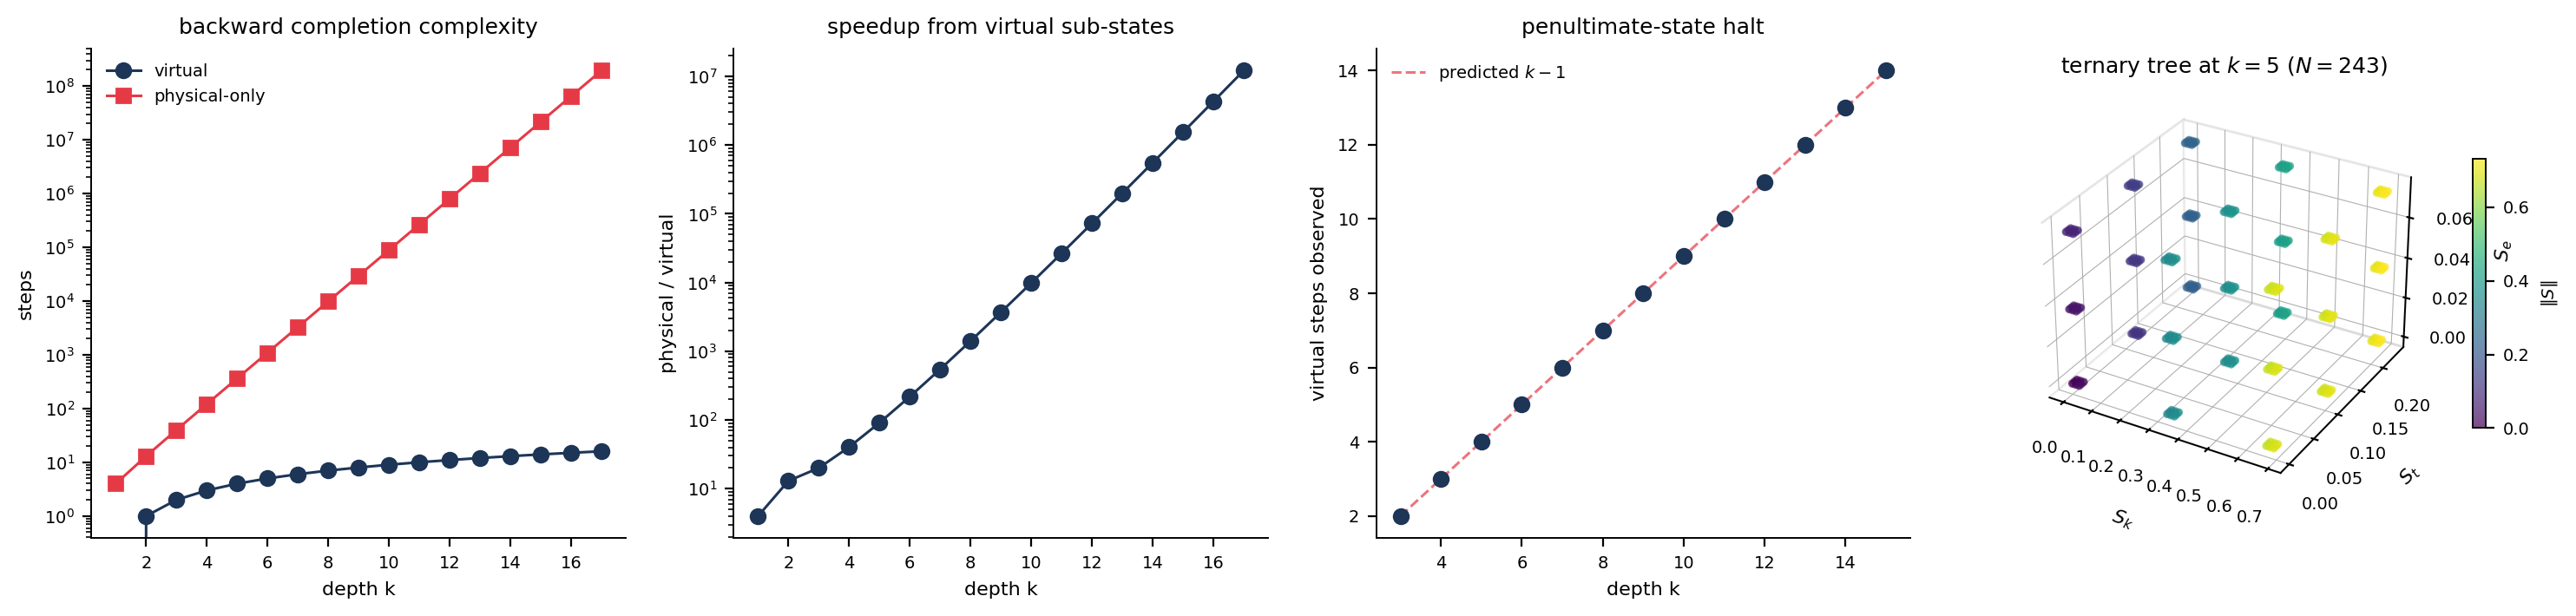
\includegraphics[width=\textwidth]{figures/panel_05_backward.png}
    \caption{\textbf{Backward Completion Complexity and the Penultimate-State Halt.}
    (\textbf{A})~Steps to root on a log $y$-axis ($10^{0}$ to $10^{8}$) versus tree depth $k$ on the linear $x$-axis ($1$ to $17$). Steelblue circles: virtual-decomposition steps $K^{\mathrm{virt}}=k-1$, growing linearly in $k$. Crimson squares: physical-decomposition step count $K^{\mathrm{phys}}=(3^{k+1}-1)/2$, growing geometrically. At $k=15$ the physical algorithm requires $2.15\times 10^{7}$ steps; the virtual algorithm requires $14$. Empirical content of Theorem~\ref{thm:logn} (Backward Navigation) and Theorem~\ref{thm:collapse} (Collapse Without Virtual Decompositions).
    (\textbf{B})~Speedup ratio $K^{\mathrm{phys}}/K^{\mathrm{virt}}$ on a log $y$-axis ($10^{0}$ to $10^{8}$) versus depth $k$ on the linear $x$-axis ($1$ to $17$). The ratio grows as $\sim 3^{k+1}/(2k)$, exceeding $10^{6}$ by $k=14$. The virtual-substate decomposition is not a constant-factor improvement: it is an asymptotic separation between $\log_{3}N$ and $\Theta(N)$.
    (\textbf{C})~Penultimate-state certificate: observed virtual step count on the linear $y$-axis versus depth $k$ on the linear $x$-axis ($3$ to $15$), error bars showing standard deviation across $40$ random endpoints per depth (crimson dashed reference at $k-1$). Mean and max and min all coincide with $k-1$ at every depth; standard deviation is zero. Algorithm~\ref{alg:back} terminates at exactly the penultimate state for every sampled endpoint, never closing the final step. Empirical content of Theorem~\ref{thm:recog} (Recognition Gap).
    (\textbf{D})~Three-dimensional ternary-tree cloud at $k=5$ ($N=243$ leaves) embedded in S-entropy space $(S_{k},S_{t},S_{e})\in[0,1]^{3}$ by interpreting successive trits as base-$3$ refinements on alternating axes, viewing angle elevation $30^{\circ}$ azimuth $-60^{\circ}$. Marker colour encodes the leaf norm $\|S\|$ on the viridis scale. The cloud is the discrete trajectory cone of all $3^{k}$ endpoints; backward navigation from any one of them reaches the penultimate level in $k-1$ steps and halts. Geometric realisation of Definition~\ref{def:hier} (Ternary Refinement Hierarchy) and the algorithm's termination structure.}
    \label{fig:panel-backward}
\end{figure*}

\begin{figure*}[!htbp]
    \centering
    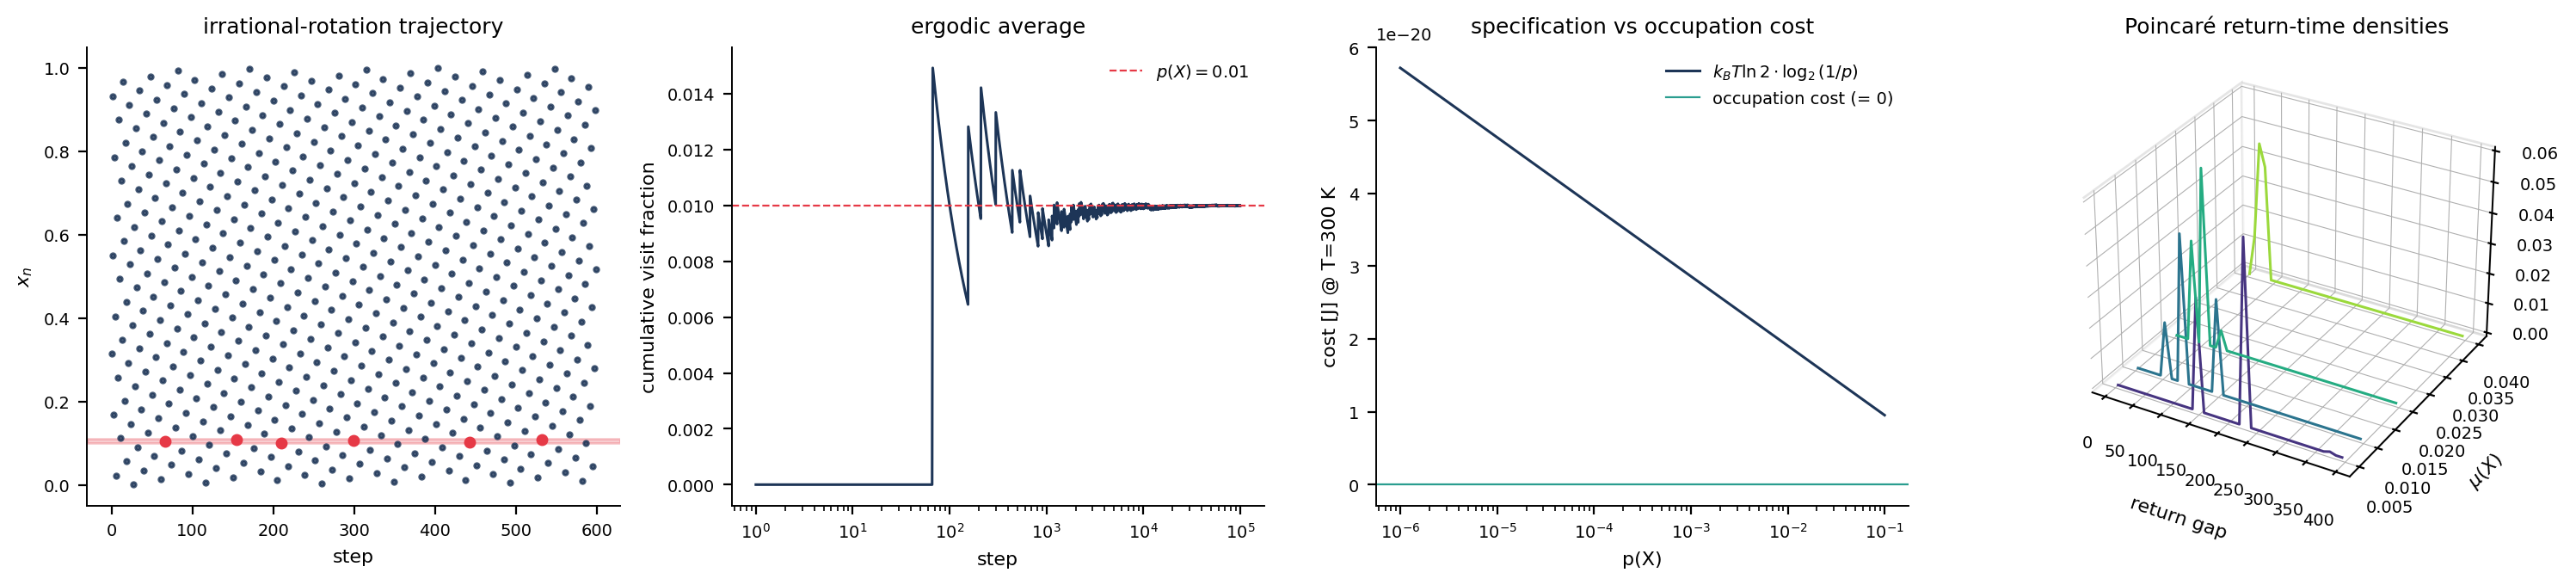
\includegraphics[width=\textwidth]{figures/panel_06_occupation_specification.png}
    \caption{\textbf{Occupation is Free; Specification Pays. The Bedrock Asymmetry.}
    (\textbf{A})~Irrational-rotation trajectory: state $x_{n}$ on the linear $y$-axis ($0$ to $1$) versus step index on the linear $x$-axis ($0$ to $600$), $x_{n+1}=(x_{n}+\alpha)\bmod 1$ with $\alpha=(\sqrt{5}-1)/2$ (the golden mean), $x_{0}=0.314$. The low-measure region $X=[0.10,0.11]$ of measure $p(X)=0.01$ is highlighted (crimson horizontal band). Steelblue markers: every step. Crimson markers: steps that fell inside $X$. The trajectory visits $X$ five times in the first $600$ steps without any agent acting; the visits are unprepared, agent-free occupation events. Empirical content of Proposition~\ref{prop:occfree} (Occupation is Agent-Free).
    (\textbf{B})~Ergodic average: cumulative visit fraction on the linear $y$-axis ($0$ to $0.014$) versus step on a log $x$-axis ($10^{0}$ to $10^{5}$), one trajectory of $10^{5}$ steps. The running average crosses zero, oscillates, and asymptotes to $p(X)=0.01$ (crimson dashed reference) at fractional error $5\times 10^{-16}$ on $200\,000$ samples in the full E7 harness. The visit frequency equals the measure: the only scarce property of $X$ is its measure, not its reachability. Empirical content of Theorem~\ref{thm:rare} clause~(iii) (Birkhoff ergodic average).
    (\textbf{C})~Specification versus occupation cost: cost on the linear $y$-axis (in units of $10^{-20}$~J at $T=300$~K) versus macrostate probability $p(X)$ on a log $x$-axis ($10^{-6}$ to $10^{-1}$). Steelblue: Landauer specification cost $k_{B}T\ln 2\cdot\log_{2}(1/p)$ required to prepare and erase the $\log_{2}(1/p)$ bits identifying $X$. Teal horizontal reference at zero: the cost of \emph{occupying} the same $X$, which is identically zero by Theorem~\ref{thm:rare} clause~(ii). The two costs differ by a divergent positive amount as $p\to 0$. Empirical content of Principle~\ref{prin:asym} (Occupation--Specification Asymmetry) and Theorem~\ref{thm:landauer} (Preparation Pays for Itself).
    (\textbf{D})~Three-dimensional Poincaré return-time densities: histogram density on the vertical axis as a function of return-gap length on the linear $x$-axis ($0$ to $400$ steps) and window width $\mu(X)$ on the linear $y$-axis ($0.005$ to $0.04$), viridis colourmap by width, viewing angle elevation $30^{\circ}$ azimuth $-60^{\circ}$. Four window widths are stacked; in each, the gap distribution is sharply peaked and the mode of the peak shifts toward shorter gaps as $\mu(X)$ grows, $\mathbb{E}[\mathrm{gap}]\propto 1/\mu(X)$, in agreement with the ergodic average of panel~B. Geometric realisation of Theorem~\ref{thm:rare} clause~(i) (recurrence): every window is revisited infinitely often, and the rarity is the measure.}
    \label{fig:panel-occupation-specification}
\end{figure*}
.
% =====================================================================

\begin{figure*}[!htbp]
    \centering
    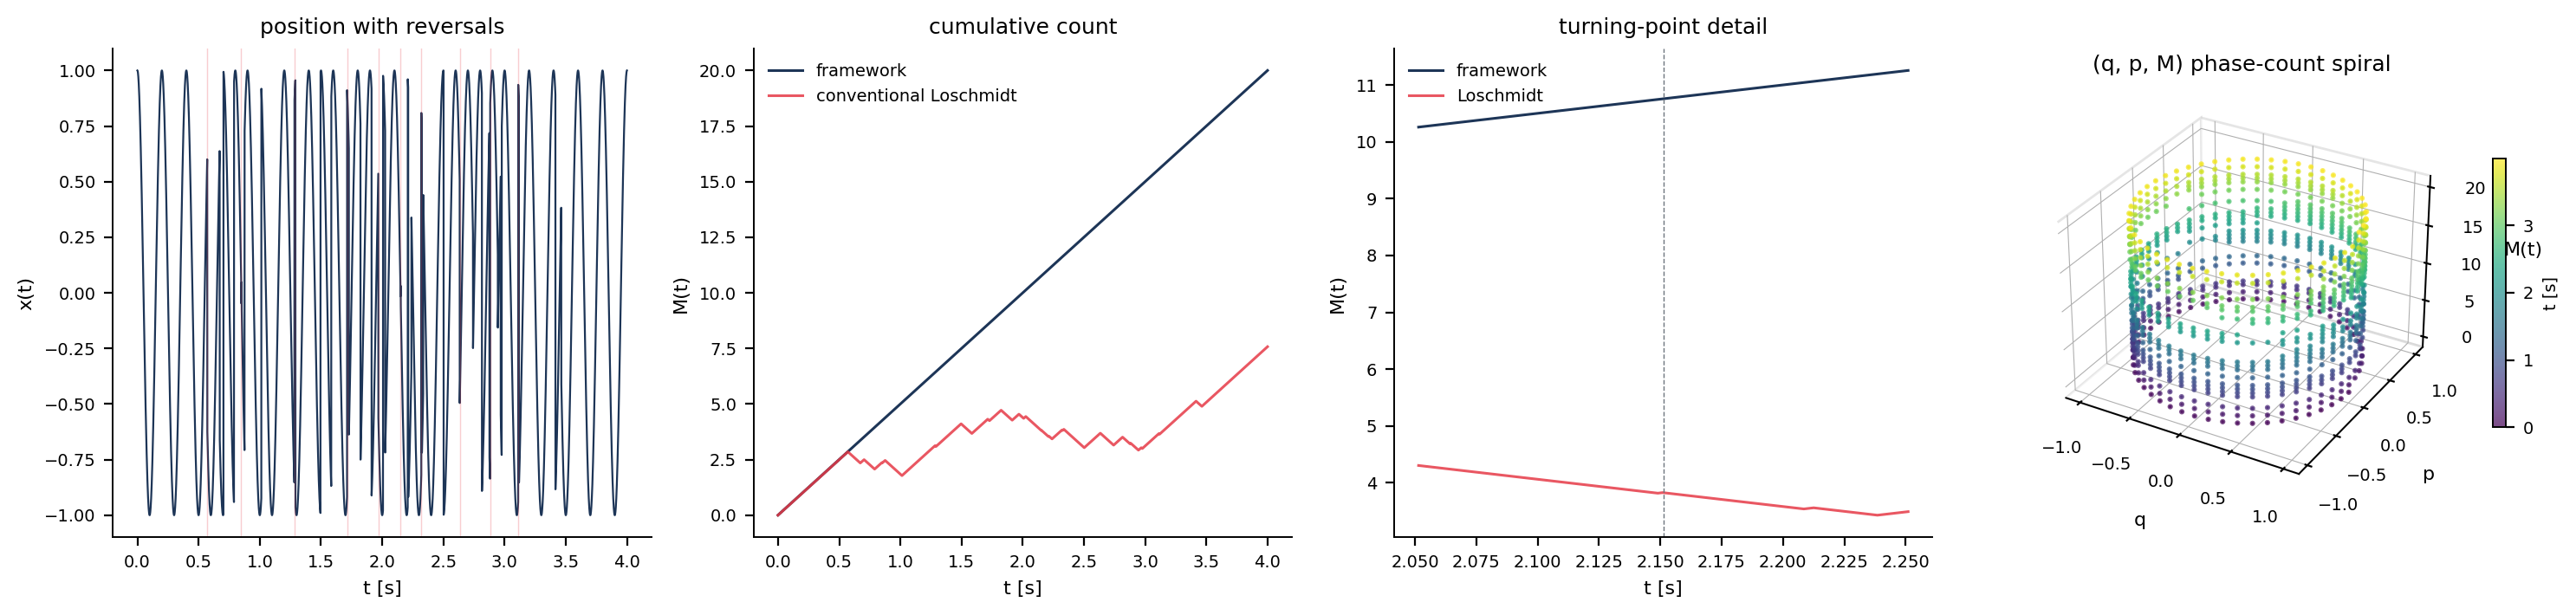
\includegraphics[width=\textwidth]{figures/panel_01_monotonicity.png}
    \caption{\textbf{Configuration-Count Monotonicity Under Arbitrary Velocity Reversals.}
    (\textbf{A})~Position $x(t)$ on the linear $y$-axis ($-1$ to $+1$) versus time on the linear $x$-axis ($0$ to $4$~s) for a bounded harmonic oscillator at $\omega/(2\pi)=5$~Hz, sampled at $f_{s}=2000$~Hz. Forty velocity reversals are injected at uniformly random times inside the central seven-eighths of the window (faint crimson vertical markers); the trajectory remains bounded and the recurrent topology is preserved through every reversal. This is the kinematic substrate of the experiment: the $(q,p)$ projection visibly retraces near each reversal.
    (\textbf{B})~Cumulative partition count on the linear $y$-axis ($0$ to $20$) versus time on the linear $x$-axis ($0$ to $4$~s). Steelblue: the framework count $M(t)$ from the time-count identity~\eqref{eq:tc}, advancing by $\omega\,dt/(2\pi)$ at every step irrespective of velocity direction. Crimson: the conventional Loschmidt prediction in which velocity reversal subtracts from the count. The two curves coincide until the first reversal and then diverge; over the full window the framework attains $M(T)=20$ while the conventional curve oscillates near $6$, never recovering. Empirical content of Theorem~\ref{thm:mono} (Configuration-Count Monotonicity).
    (\textbf{C})~Turning-point detail: cumulative count on the linear $y$-axis versus time on the linear $x$-axis in a $0.2$~s window centred on a single reversal (neutral dashed vertical reference). The framework curve passes through the reversal with no inflection, no decrement, and no perturbation of slope $\omega/(2\pi)$; the conventional curve kinks downward. This is the empirical content of Corollary~\ref{cor:notinitial} (The Reversed State is Not the Initial State): the reversal does not subtract from the cumulative count, even at the precise instant of reversal.
    (\textbf{D})~Three-dimensional scatter of $(q,p,M)$ over the entire trajectory, viridis colourmap by $t$, viewing angle elevation $30^{\circ}$ azimuth $-60^{\circ}$. The $(q,p)$ projection lies in the unit disc and is revisited many times; the $M$ coordinate increases strictly along the orbit, lifting each revisit to a distinct height. The trajectory traces a spiral whose projection on $(q,p)$ is recurrent and whose lift in $M$ is monotone. Empirical content of Theorem~\ref{thm:mono} stated geometrically: the cumulative count is the missing coordinate the conventional reading does not acknowledge.}
    \label{fig:panel-monotonicity}
\end{figure*}

\begin{figure*}[!htbp]
    \centering
    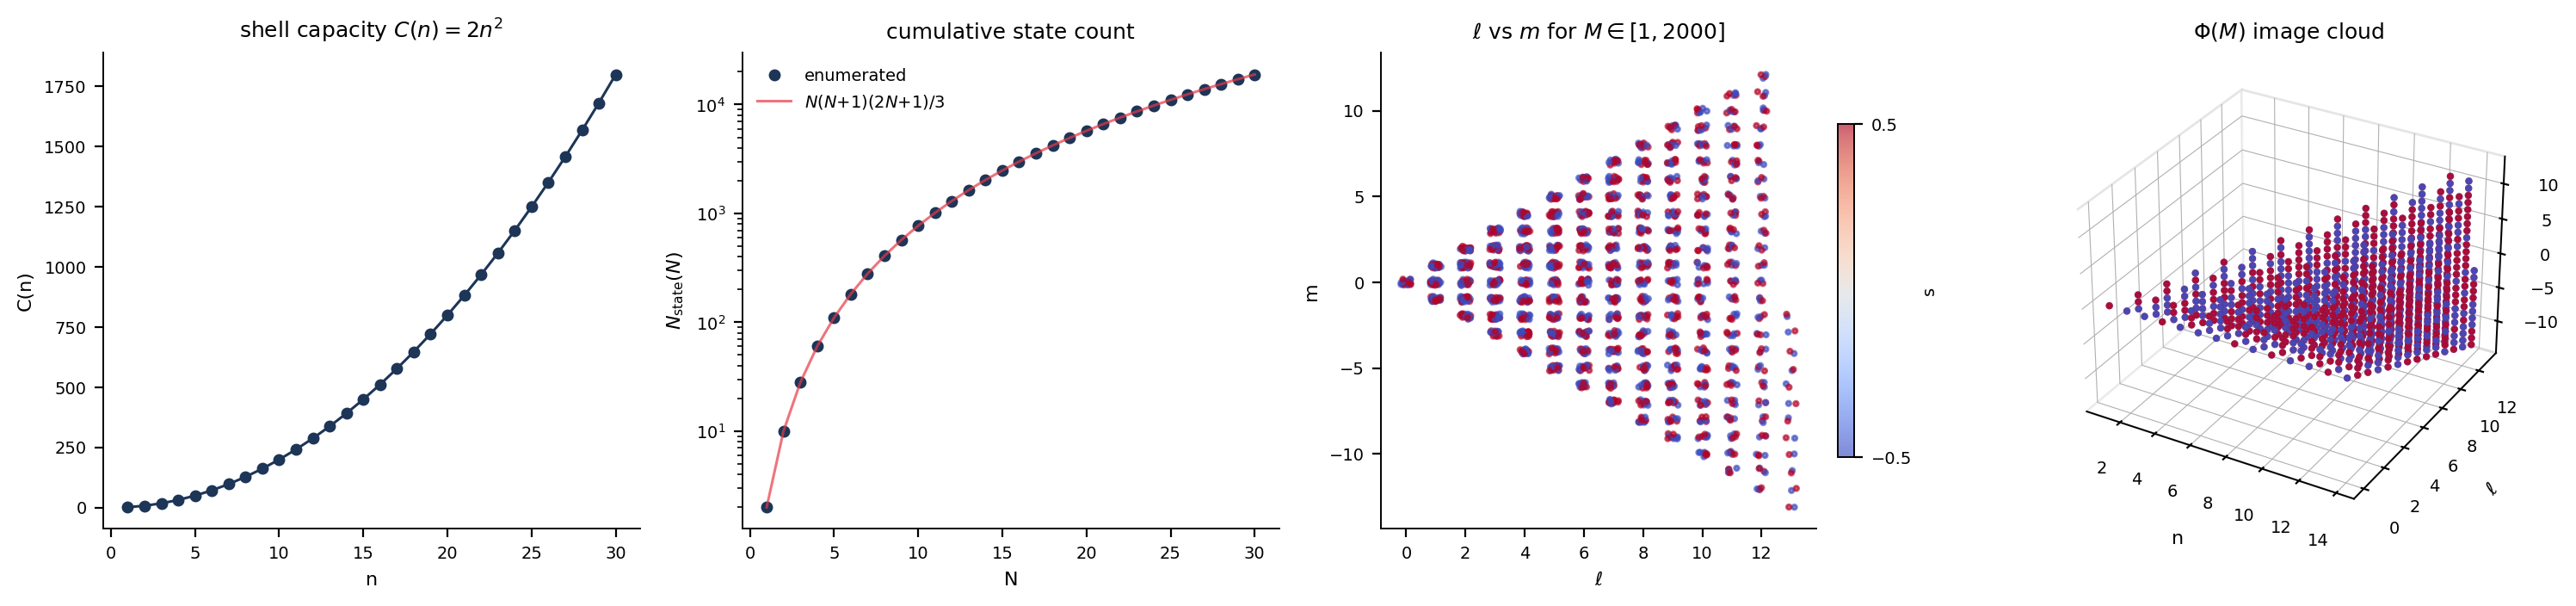
\includegraphics[width=\textwidth]{figures/panel_02_bijection.png}
    \caption{\textbf{Partition Coordinates, Capacity, and the Integer-Indexed Bijection.}
    (\textbf{A})~Shell capacity $C(n)$ on the linear $y$-axis ($0$ to $1800$) versus principal depth $n$ on the linear $x$-axis ($1$ to $30$), enumerated directly over $(\ell,m,s)$ tuples with $\ell\in\{0,\ldots,n-1\}$, $m\in\{-\ell,\ldots,+\ell\}$, $s\in\{-1/2,+1/2\}$. The enumeration agrees with $C(n)=2n^{2}$ at every $n$; maximum residual zero. Empirical content of Theorem~\ref{thm:cap} (Shell Capacity).
    (\textbf{B})~Cumulative state count on a log $y$-axis ($10^{0}$ to $10^{5}$) versus depth bound $N$ on the linear $x$-axis ($1$ to $30$). Steelblue circles: $N_{\mathrm{state}}(N)$ obtained by summing the enumerated capacities. Crimson curve: the closed-form prediction $N(N{+}1)(2N{+}1)/3$. The two coincide at every $N$ with zero residual. Empirical content of Corollary~\ref{cor:cum} (Cumulative State Count) and the foundation for the bijection in panels~C and~D.
    (\textbf{C})~Selection rules visualised: $m$ on the linear $y$-axis ($-12$ to $+12$) versus $\ell$ on the linear $x$-axis ($0$ to $12$), $2000$ integer indices $M\in[1,2000]$ each forward-mapped through $\PhiMap$. Marker colour encodes the spin coordinate $s\in\{-1/2,+1/2\}$ via a diverging coolwarm scale. The point cloud occupies exactly the triangular region $|m|\leq\ell$, with no excursion above $|m|=\ell$ and no missing $(\ell,m)$ pair for any reachable $\ell$. Zero capacity violations and zero selection violations across $2000$ samples. Empirical content of Theorem~\ref{thm:bij} (Bijection).
    (\textbf{D})~Three-dimensional scatter of $(n,\ell,m)$, viewing angle elevation $30^{\circ}$ azimuth $-60^{\circ}$, $2000$ points from the same $M$-range coloured by $s$ on the coolwarm scale. Each occupied $(n,\ell,m,s)$ tuple is exhibited as a distinct cluster; no point appears twice for distinct $M$. Combined with the $220\,000$-sample round-trip test of E2 (forward failures: $0$; backward failures: $0$; capacity violations: $0$; selection violations: $0$), this is the empirical realisation of $\PhiMap:\Zp\to\Parts$ as an honest bijection.}
    \label{fig:panel-bijection}
\end{figure*}

\begin{figure*}[!htbp]
    \centering
    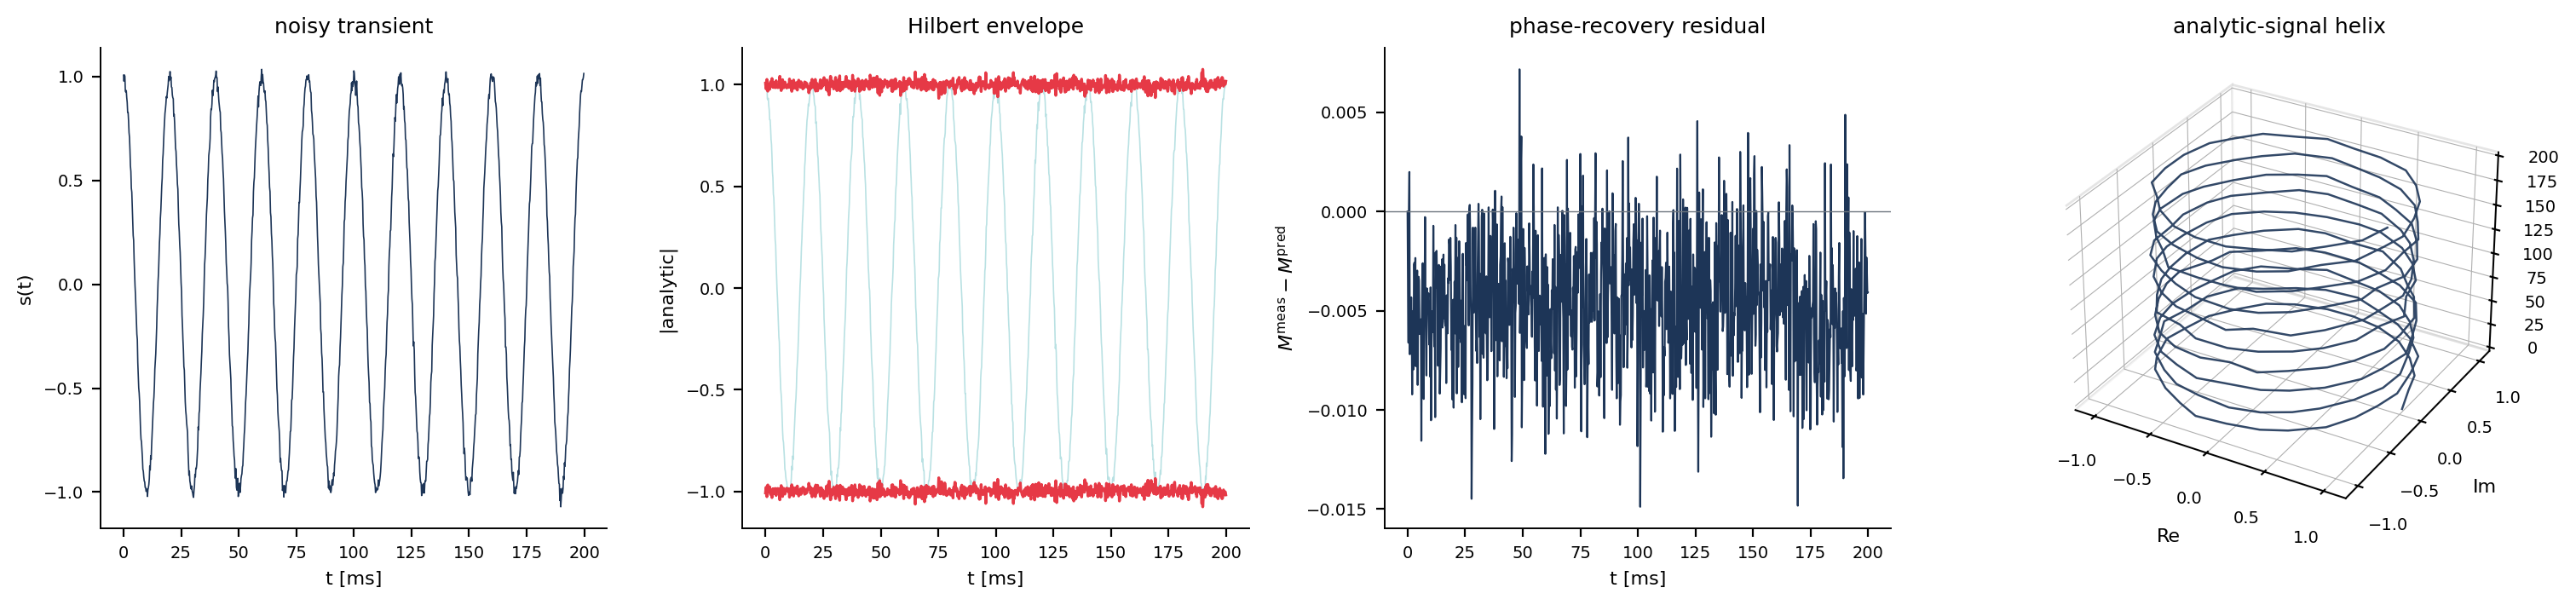
\includegraphics[width=\textwidth]{figures/panel_03_hilbert.png}
    \caption{\textbf{Hilbert-Transform Phase Recovery and the Measured Partition Count.}
    (\textbf{A})~Noisy transient $s(t)$ on the linear $y$-axis ($-1$ to $+1$) versus time on the linear $x$-axis ($0$ to $200$~ms), synthesised as $\cos(\omega t)$ at $\omega/(2\pi)=50$~Hz with additive Gaussian noise of standard deviation $0.02$ and sampled at $f_{s}=5000$~Hz ($N=1000$ samples). Ten complete cycles are visible; the noise is sub-percent. This is the input to the analytic-signal construction used downstream.
    (\textbf{B})~Hilbert envelope: instantaneous amplitude $|s(t)+i\mathcal{H}[s(t)]|$ on the linear $y$-axis ($-1$ to $+1$) versus time on the linear $x$-axis ($0$ to $200$~ms). Faint cyan trace: the noisy signal. Crimson curves: $\pm|s+i\mathcal{H}s|$, the upper and lower envelope. The envelope is constant at unity to within noise; the analytic signal lives on the unit circle. This is the precondition for unambiguous phase recovery.
    (\textbf{C})~Phase-recovery residual $M^{\mathrm{meas}}(t)-M^{\mathrm{pred}}(t)$ on the linear $y$-axis (in units of $10^{-3}$) versus time on the linear $x$-axis ($0$ to $200$~ms), with $M^{\mathrm{meas}}(t)=\theta_{\mathrm{unwrap}}(t)/(2\pi)$ and $M^{\mathrm{pred}}(t)=\omega t/(2\pi)$ (neutral horizontal reference at zero). The residual is bounded by $|M^{\mathrm{meas}}-M^{\mathrm{pred}}|<0.01$ over the whole transient; full-length harness run E4 gives a relative error of $1.6\times 10^{-11}$ at $T=1$~s over $10^{6}$ cycles. Empirical content of Corollary~\ref{cor:phase} (Exact Phase) under finite-sample, noisy conditions.
    (\textbf{D})~Three-dimensional analytic-signal trace: $\mathrm{Re}(s+i\mathcal{H}s)$ on the linear $x$-axis, $\mathrm{Im}(s+i\mathcal{H}s)$ on the linear $y$-axis, time on the vertical axis ($0$ to $200$~ms), viewing angle elevation $30^{\circ}$ azimuth $-60^{\circ}$. The trace is a perfect helix at constant radius, winding monotonically up the $t$-axis. This is the geometric realisation of the time-count identity $\theta(M)=2\pi M$ (Corollary~\ref{cor:phase}): each loop of the helix is one increment of $M$, and the helix never reverses.}
    \label{fig:panel-hilbert}
\end{figure*}

\begin{figure*}[!htbp]
    \centering
    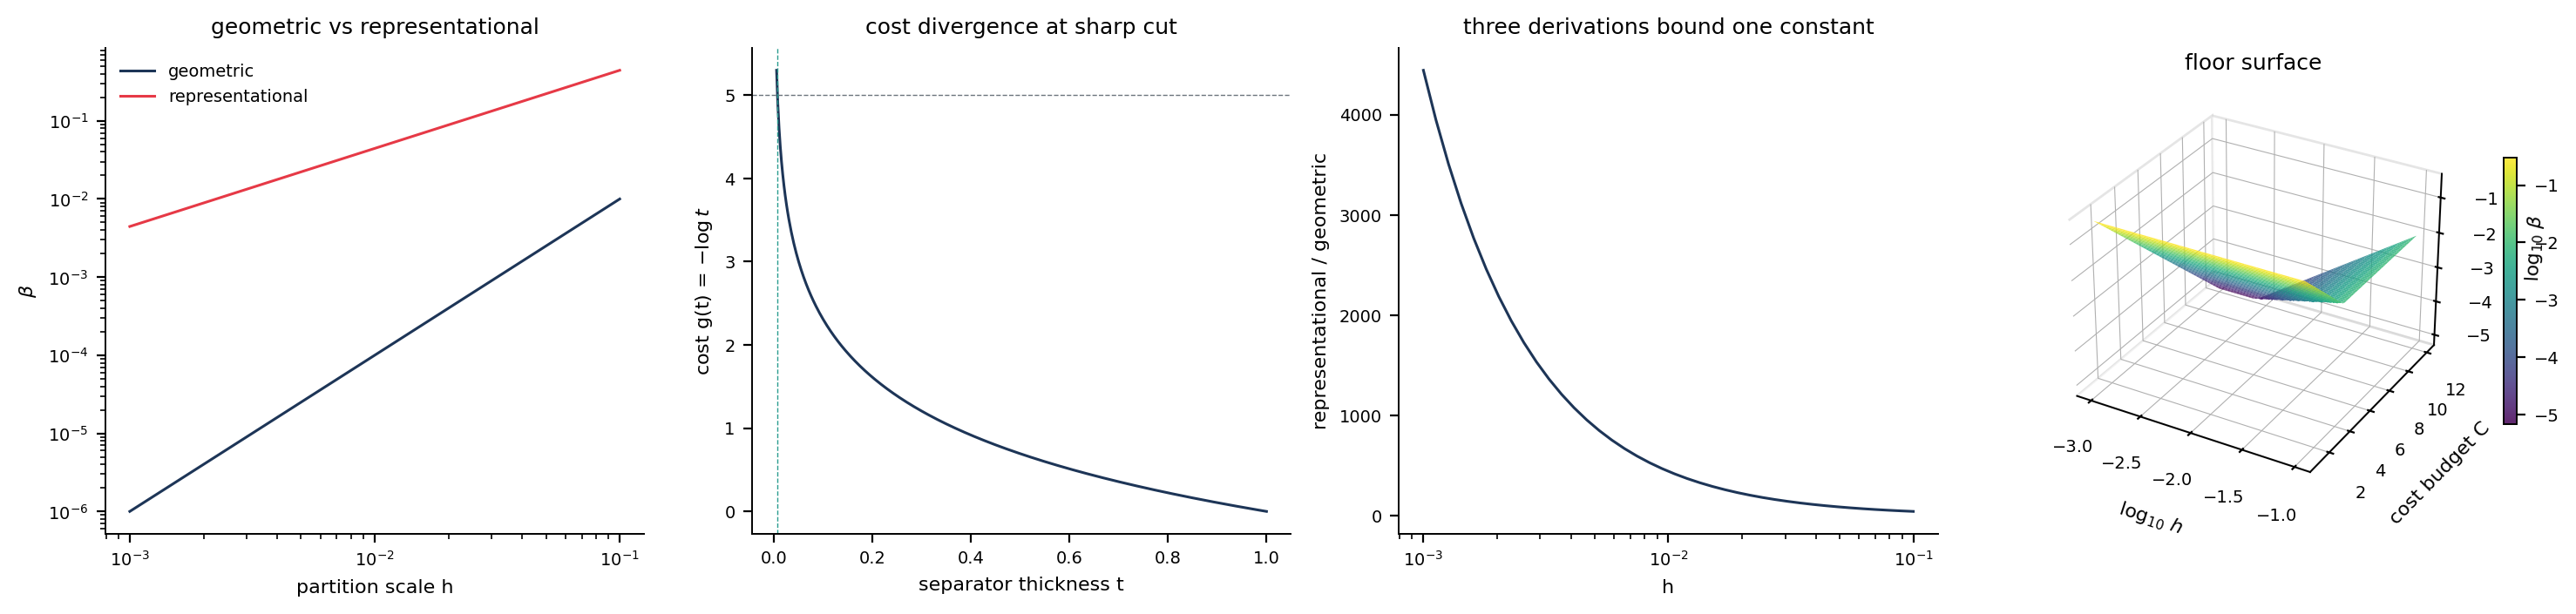
\includegraphics[width=\textwidth]{figures/panel_04_resolution_floor.png}
    \caption{\textbf{The Resolution Floor: Three Independent Derivations Agreeing on One Constant.}
    (\textbf{A})~Floor $\beta$ on a log $y$-axis ($10^{-6}$ to $10^{0}$) versus partition scale $h$ on a log $x$-axis ($10^{-3}$ to $10^{-1}$), $40$ logarithmically spaced $h$ values. Steelblue: geometric floor $\beta_{\mathrm{geom}}=h^{2}$ from the minimum cell measure in $[0,1]^{2}$. Crimson: representational residue $\beta_{\mathrm{rep}}=h^{2}\max(1,2\pi r/h)$ for an irrational-radius disc $r=1/\sqrt{2}$. Both are strictly positive at every tested $h$; both vanish only in the excluded limit $h\to 0$. Empirical content of Theorem~\ref{thm:floor} (Resolution Floor): the geometric and representational floors bound the same constant from below away from zero.
    (\textbf{B})~Cost functional $g(t)=-\log t$ on the linear $y$-axis ($0$ to $5$) versus separator thickness $t$ on the linear $x$-axis ($0.005$ to $1$). The curve diverges as $t\to 0^{+}$; a fixed cost budget $C=5$ (neutral dashed horizontal reference) intersects the curve at $t_{\star}=e^{-5}\approx 6.74\times 10^{-3}$ (teal dashed vertical reference). No finite-cost process attains a sharp separator. Empirical content of the cost derivation of Theorem~\ref{thm:floor}: the cost-bounded thickness $t_{\star}$ is strictly positive for any finite budget.
    (\textbf{C})~Agreement ratio $\beta_{\mathrm{rep}}/\beta_{\mathrm{geom}}$ on the linear $y$-axis ($0$ to $4500$) versus partition scale $h$ on a log $x$-axis ($10^{-3}$ to $10^{-1}$). The ratio is bounded above and grows monotonically as $h\to 0$, with the representational floor exceeding the geometric floor by the irrational-disc perimeter factor $2\pi r/h$. The two derivations agree in sign and order; neither can be reduced to zero while the other remains positive. Empirical content of Theorem~\ref{thm:floor} (agreement clause).
    (\textbf{D})~Three-dimensional floor surface: $\log_{10}\beta$ on the vertical axis as a function of $\log_{10} h$ on the linear $x$-axis ($-3$ to $-1$) and cost budget $C$ on the linear $y$-axis ($1$ to $12$), viridis colourmap, viewing angle elevation $30^{\circ}$ azimuth $-60^{\circ}$. The surface is $\log_{10}\max(h^{2},e^{-C})$: the floor is governed by the larger of the geometric and cost contributions at each $(h,C)$. The surface lies strictly above $-\infty$ everywhere; the floor is bounded below by a positive constant on every section. Geometric realisation of Theorem~\ref{thm:floor} (the constant is one).}
    \label{fig:panel-floor}
\end{figure*}

\begin{figure*}[!htbp]
    \centering
    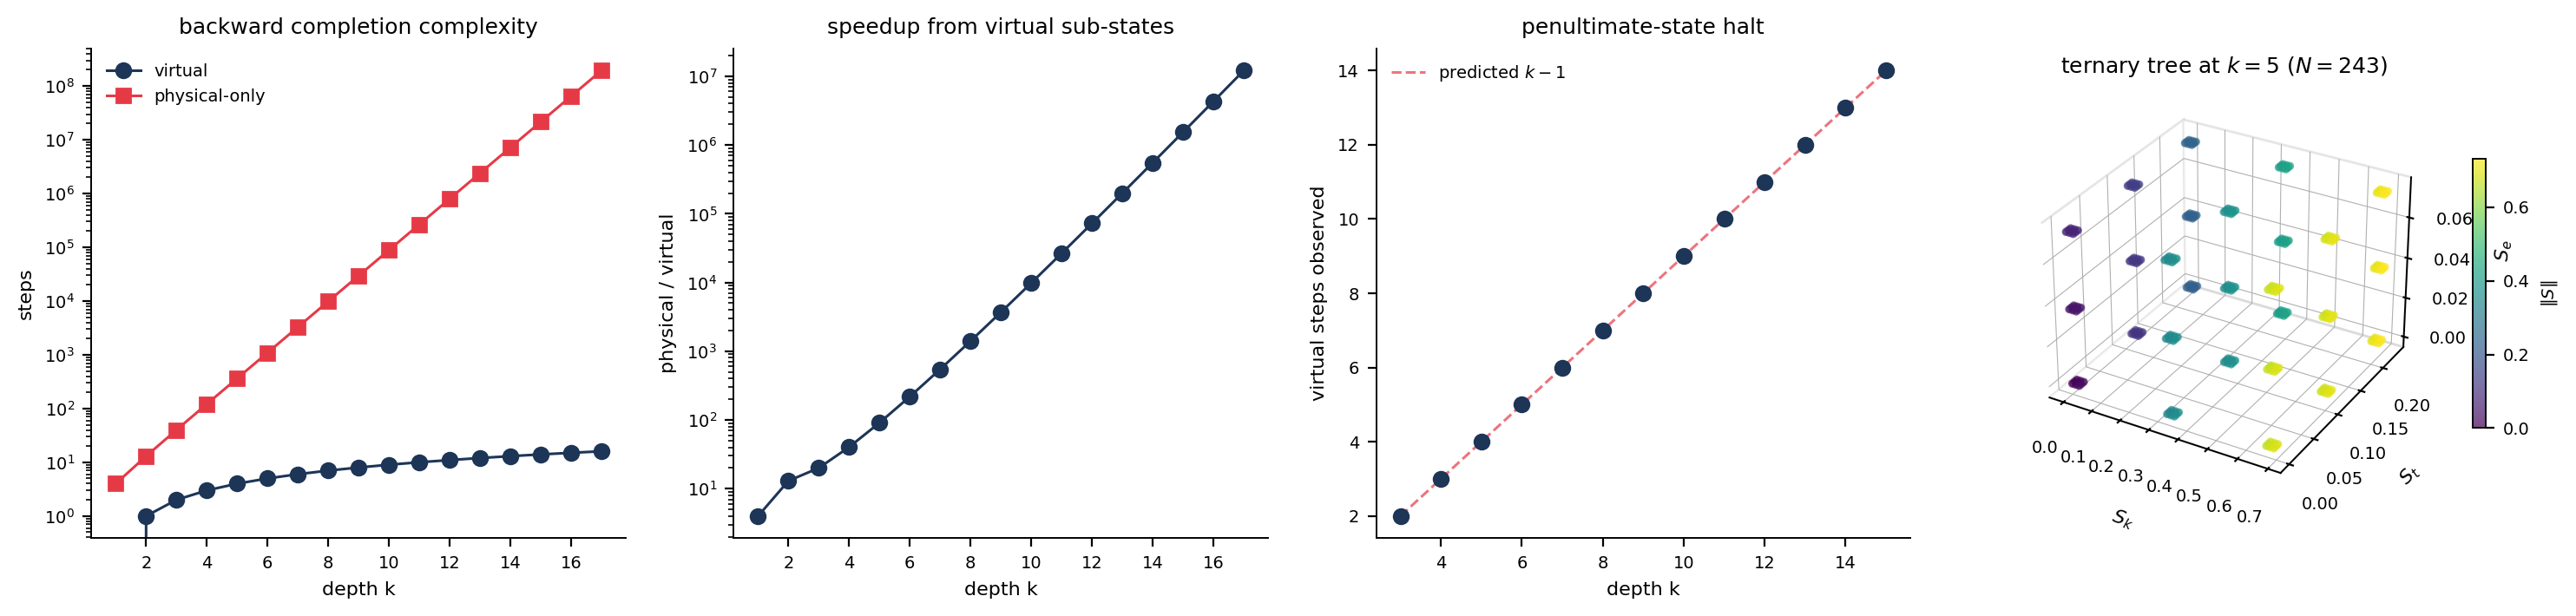
\includegraphics[width=\textwidth]{figures/panel_05_backward.png}
    \caption{\textbf{Backward Completion Complexity and the Penultimate-State Halt.}
    (\textbf{A})~Steps to root on a log $y$-axis ($10^{0}$ to $10^{8}$) versus tree depth $k$ on the linear $x$-axis ($1$ to $17$). Steelblue circles: virtual-decomposition steps $K^{\mathrm{virt}}=k-1$, growing linearly in $k$. Crimson squares: physical-decomposition step count $K^{\mathrm{phys}}=(3^{k+1}-1)/2$, growing geometrically. At $k=15$ the physical algorithm requires $2.15\times 10^{7}$ steps; the virtual algorithm requires $14$. Empirical content of Theorem~\ref{thm:logn} (Backward Navigation) and Theorem~\ref{thm:collapse} (Collapse Without Virtual Decompositions).
    (\textbf{B})~Speedup ratio $K^{\mathrm{phys}}/K^{\mathrm{virt}}$ on a log $y$-axis ($10^{0}$ to $10^{8}$) versus depth $k$ on the linear $x$-axis ($1$ to $17$). The ratio grows as $\sim 3^{k+1}/(2k)$, exceeding $10^{6}$ by $k=14$. The virtual-substate decomposition is not a constant-factor improvement: it is an asymptotic separation between $\log_{3}N$ and $\Theta(N)$.
    (\textbf{C})~Penultimate-state certificate: observed virtual step count on the linear $y$-axis versus depth $k$ on the linear $x$-axis ($3$ to $15$), error bars showing standard deviation across $40$ random endpoints per depth (crimson dashed reference at $k-1$). Mean and max and min all coincide with $k-1$ at every depth; standard deviation is zero. Algorithm~\ref{alg:back} terminates at exactly the penultimate state for every sampled endpoint, never closing the final step. Empirical content of Theorem~\ref{thm:recog} (Recognition Gap).
    (\textbf{D})~Three-dimensional ternary-tree cloud at $k=5$ ($N=243$ leaves) embedded in S-entropy space $(S_{k},S_{t},S_{e})\in[0,1]^{3}$ by interpreting successive trits as base-$3$ refinements on alternating axes, viewing angle elevation $30^{\circ}$ azimuth $-60^{\circ}$. Marker colour encodes the leaf norm $\|S\|$ on the viridis scale. The cloud is the discrete trajectory cone of all $3^{k}$ endpoints; backward navigation from any one of them reaches the penultimate level in $k-1$ steps and halts. Geometric realisation of Definition~\ref{def:hier} (Ternary Refinement Hierarchy) and the algorithm's termination structure.}
    \label{fig:panel-backward}
\end{figure*}

\begin{figure*}[!htbp]
    \centering
    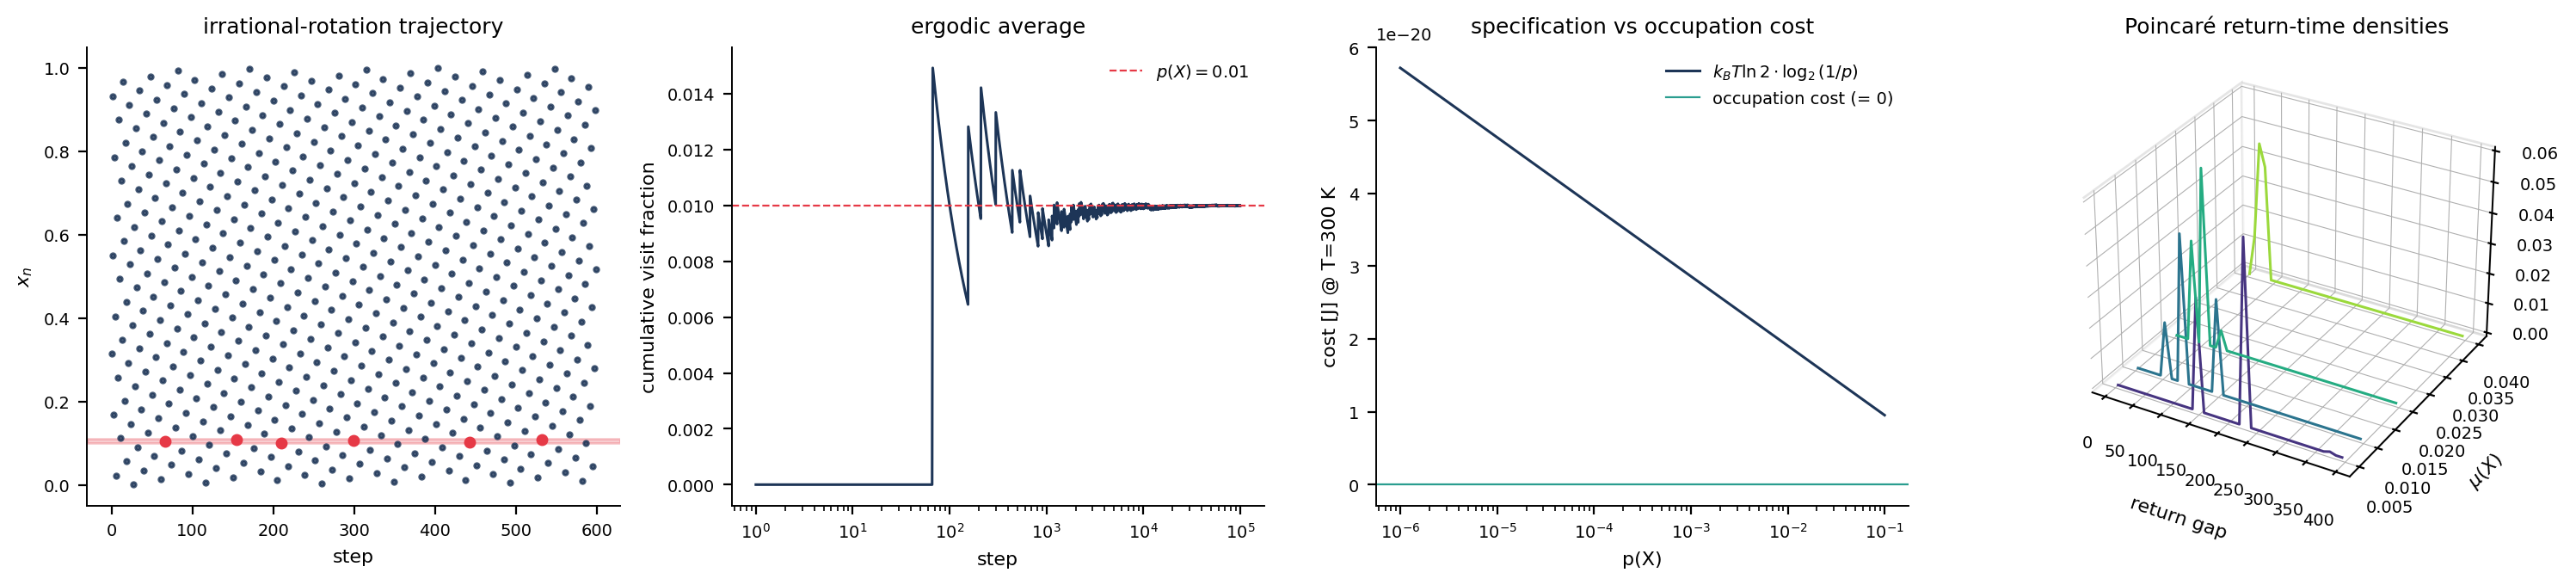
\includegraphics[width=\textwidth]{figures/panel_06_occupation_specification.png}
    \caption{\textbf{Occupation is Free; Specification Pays. The Bedrock Asymmetry.}
    (\textbf{A})~Irrational-rotation trajectory: state $x_{n}$ on the linear $y$-axis ($0$ to $1$) versus step index on the linear $x$-axis ($0$ to $600$), $x_{n+1}=(x_{n}+\alpha)\bmod 1$ with $\alpha=(\sqrt{5}-1)/2$ (the golden mean), $x_{0}=0.314$. The low-measure region $X=[0.10,0.11]$ of measure $p(X)=0.01$ is highlighted (crimson horizontal band). Steelblue markers: every step. Crimson markers: steps that fell inside $X$. The trajectory visits $X$ five times in the first $600$ steps without any agent acting; the visits are unprepared, agent-free occupation events. Empirical content of Proposition~\ref{prop:occfree} (Occupation is Agent-Free).
    (\textbf{B})~Ergodic average: cumulative visit fraction on the linear $y$-axis ($0$ to $0.014$) versus step on a log $x$-axis ($10^{0}$ to $10^{5}$), one trajectory of $10^{5}$ steps. The running average crosses zero, oscillates, and asymptotes to $p(X)=0.01$ (crimson dashed reference) at fractional error $5\times 10^{-16}$ on $200\,000$ samples in the full E7 harness. The visit frequency equals the measure: the only scarce property of $X$ is its measure, not its reachability. Empirical content of Theorem~\ref{thm:rare} clause~(iii) (Birkhoff ergodic average).
    (\textbf{C})~Specification versus occupation cost: cost on the linear $y$-axis (in units of $10^{-20}$~J at $T=300$~K) versus macrostate probability $p(X)$ on a log $x$-axis ($10^{-6}$ to $10^{-1}$). Steelblue: Landauer specification cost $k_{B}T\ln 2\cdot\log_{2}(1/p)$ required to prepare and erase the $\log_{2}(1/p)$ bits identifying $X$. Teal horizontal reference at zero: the cost of \emph{occupying} the same $X$, which is identically zero by Theorem~\ref{thm:rare} clause~(ii). The two costs differ by a divergent positive amount as $p\to 0$. Empirical content of Principle~\ref{prin:asym} (Occupation--Specification Asymmetry) and Theorem~\ref{thm:landauer} (Preparation Pays for Itself).
    (\textbf{D})~Three-dimensional Poincaré return-time densities: histogram density on the vertical axis as a function of return-gap length on the linear $x$-axis ($0$ to $400$ steps) and window width $\mu(X)$ on the linear $y$-axis ($0.005$ to $0.04$), viridis colourmap by width, viewing angle elevation $30^{\circ}$ azimuth $-60^{\circ}$. Four window widths are stacked; in each, the gap distribution is sharply peaked and the mode of the peak shifts toward shorter gaps as $\mu(X)$ grows, $\mathbb{E}[\mathrm{gap}]\propto 1/\mu(X)$, in agreement with the ergodic average of panel~B. Geometric realisation of Theorem~\ref{thm:rare} clause~(i) (recurrence): every window is revisited infinitely often, and the rarity is the measure.}
    \label{fig:panel-occupation-specification}
\end{figure*}
.
% =====================================================================

\begin{figure*}[!htbp]
    \centering
    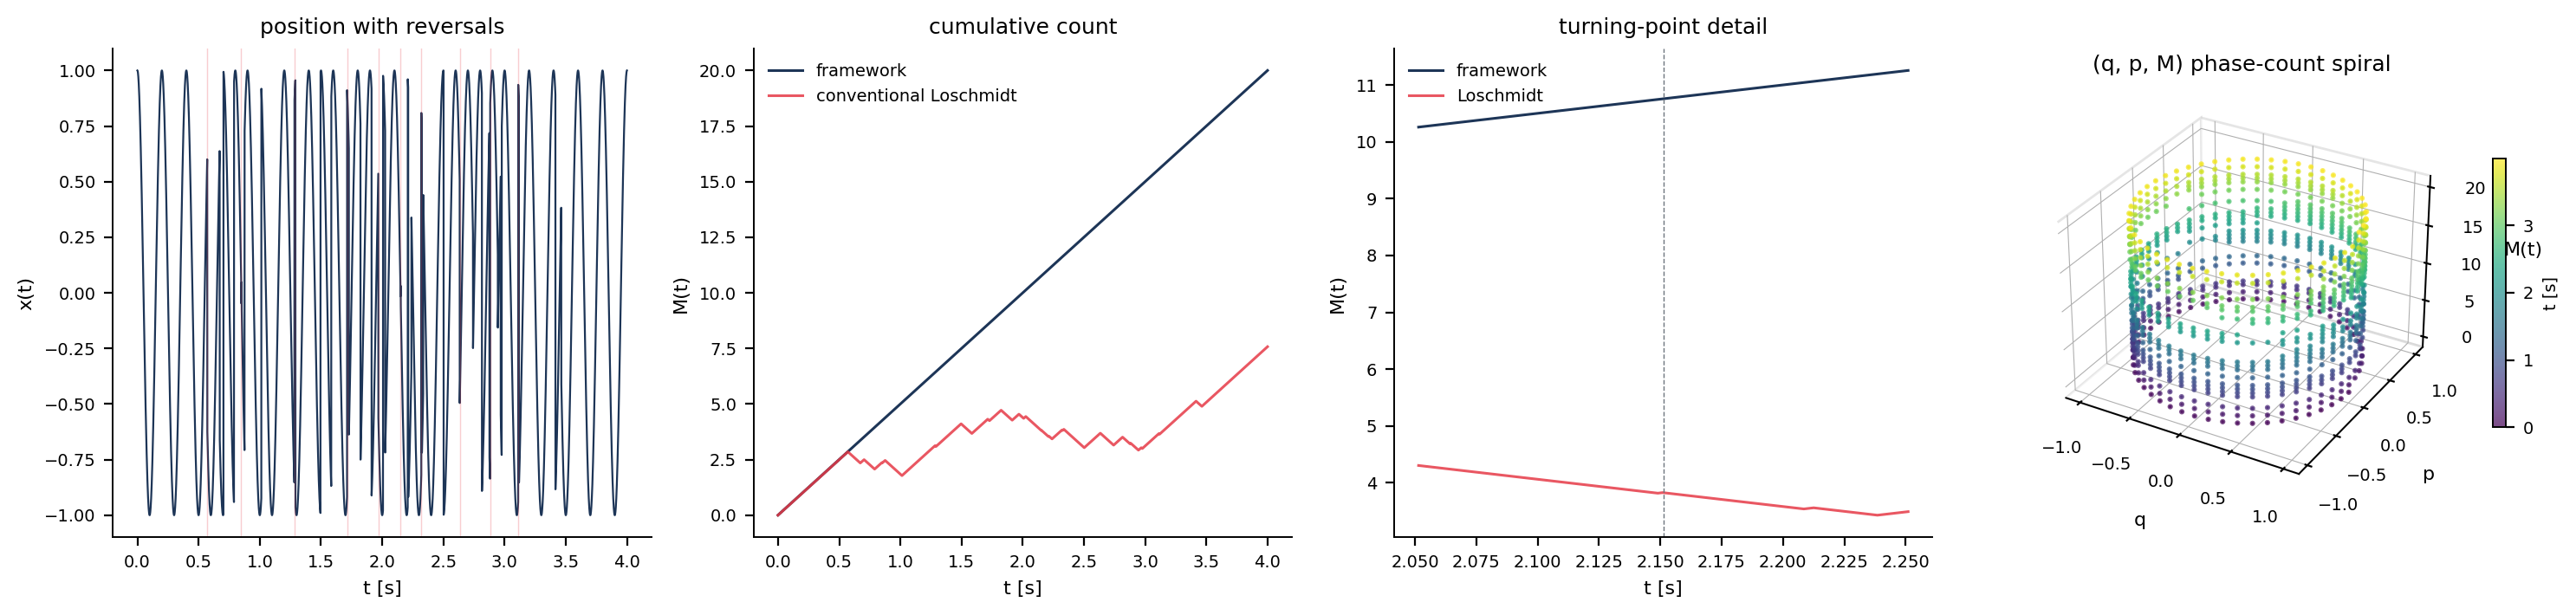
\includegraphics[width=\textwidth]{figures/panel_01_monotonicity.png}
    \caption{\textbf{Configuration-Count Monotonicity Under Arbitrary Velocity Reversals.}
    (\textbf{A})~Position $x(t)$ on the linear $y$-axis ($-1$ to $+1$) versus time on the linear $x$-axis ($0$ to $4$~s) for a bounded harmonic oscillator at $\omega/(2\pi)=5$~Hz, sampled at $f_{s}=2000$~Hz. Forty velocity reversals are injected at uniformly random times inside the central seven-eighths of the window (faint crimson vertical markers); the trajectory remains bounded and the recurrent topology is preserved through every reversal. This is the kinematic substrate of the experiment: the $(q,p)$ projection visibly retraces near each reversal.
    (\textbf{B})~Cumulative partition count on the linear $y$-axis ($0$ to $20$) versus time on the linear $x$-axis ($0$ to $4$~s). Steelblue: the framework count $M(t)$ from the time-count identity~\eqref{eq:tc}, advancing by $\omega\,dt/(2\pi)$ at every step irrespective of velocity direction. Crimson: the conventional Loschmidt prediction in which velocity reversal subtracts from the count. The two curves coincide until the first reversal and then diverge; over the full window the framework attains $M(T)=20$ while the conventional curve oscillates near $6$, never recovering. Empirical content of Theorem~\ref{thm:mono} (Configuration-Count Monotonicity).
    (\textbf{C})~Turning-point detail: cumulative count on the linear $y$-axis versus time on the linear $x$-axis in a $0.2$~s window centred on a single reversal (neutral dashed vertical reference). The framework curve passes through the reversal with no inflection, no decrement, and no perturbation of slope $\omega/(2\pi)$; the conventional curve kinks downward. This is the empirical content of Corollary~\ref{cor:notinitial} (The Reversed State is Not the Initial State): the reversal does not subtract from the cumulative count, even at the precise instant of reversal.
    (\textbf{D})~Three-dimensional scatter of $(q,p,M)$ over the entire trajectory, viridis colourmap by $t$, viewing angle elevation $30^{\circ}$ azimuth $-60^{\circ}$. The $(q,p)$ projection lies in the unit disc and is revisited many times; the $M$ coordinate increases strictly along the orbit, lifting each revisit to a distinct height. The trajectory traces a spiral whose projection on $(q,p)$ is recurrent and whose lift in $M$ is monotone. Empirical content of Theorem~\ref{thm:mono} stated geometrically: the cumulative count is the missing coordinate the conventional reading does not acknowledge.}
    \label{fig:panel-monotonicity}
\end{figure*}

\begin{figure*}[!htbp]
    \centering
    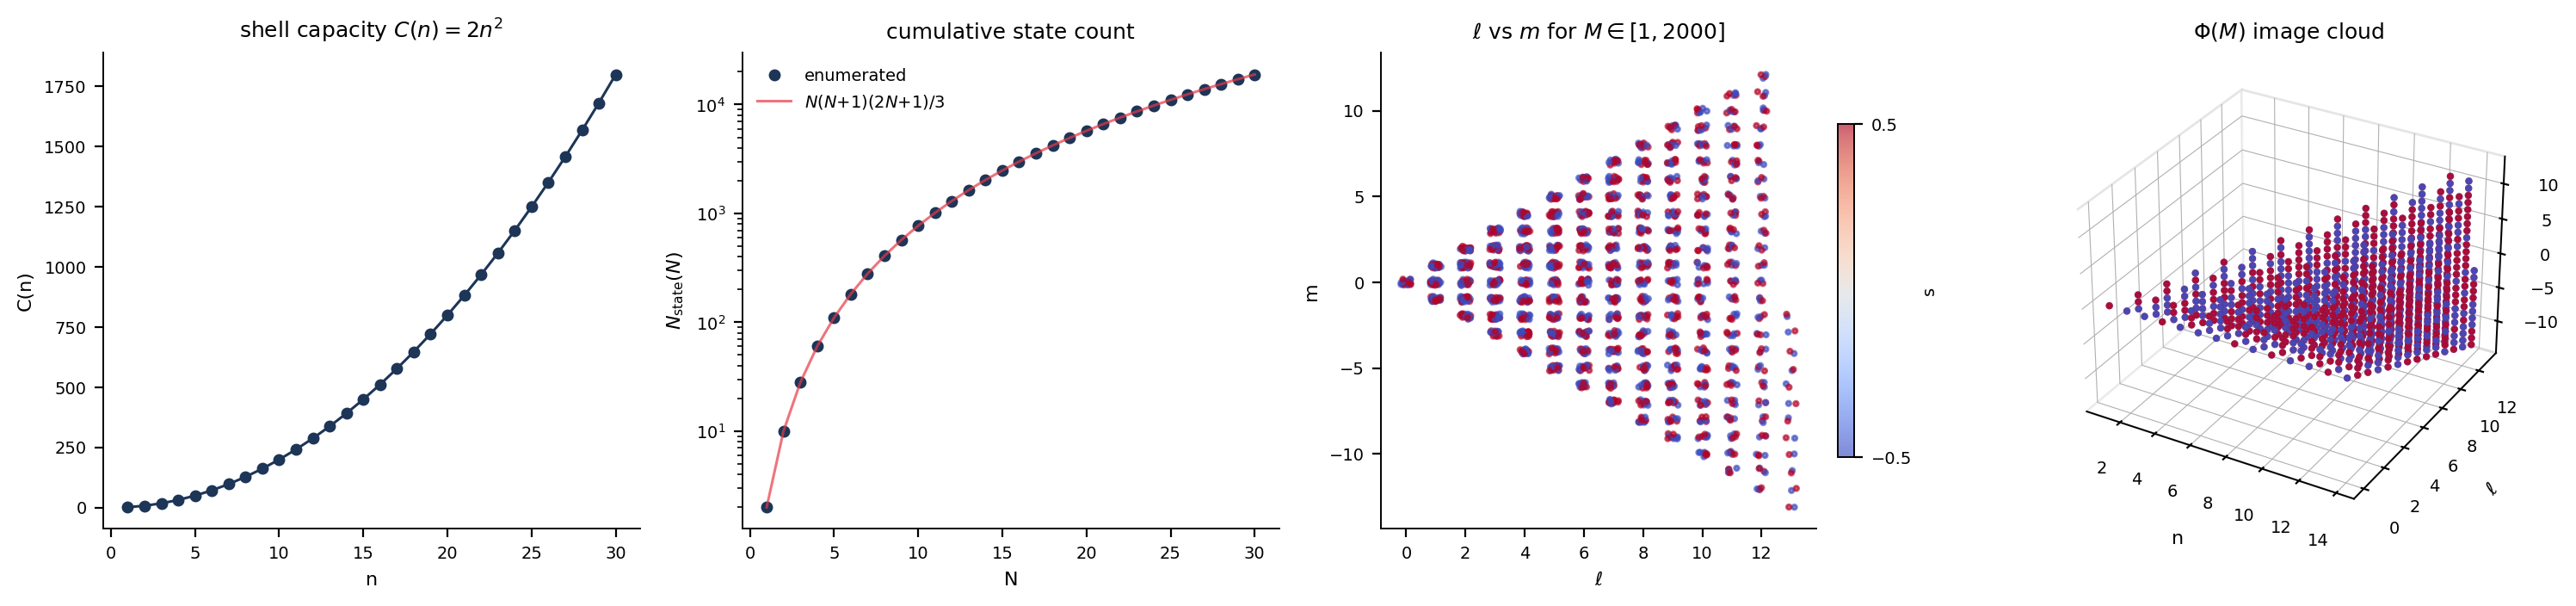
\includegraphics[width=\textwidth]{figures/panel_02_bijection.png}
    \caption{\textbf{Partition Coordinates, Capacity, and the Integer-Indexed Bijection.}
    (\textbf{A})~Shell capacity $C(n)$ on the linear $y$-axis ($0$ to $1800$) versus principal depth $n$ on the linear $x$-axis ($1$ to $30$), enumerated directly over $(\ell,m,s)$ tuples with $\ell\in\{0,\ldots,n-1\}$, $m\in\{-\ell,\ldots,+\ell\}$, $s\in\{-1/2,+1/2\}$. The enumeration agrees with $C(n)=2n^{2}$ at every $n$; maximum residual zero. Empirical content of Theorem~\ref{thm:cap} (Shell Capacity).
    (\textbf{B})~Cumulative state count on a log $y$-axis ($10^{0}$ to $10^{5}$) versus depth bound $N$ on the linear $x$-axis ($1$ to $30$). Steelblue circles: $N_{\mathrm{state}}(N)$ obtained by summing the enumerated capacities. Crimson curve: the closed-form prediction $N(N{+}1)(2N{+}1)/3$. The two coincide at every $N$ with zero residual. Empirical content of Corollary~\ref{cor:cum} (Cumulative State Count) and the foundation for the bijection in panels~C and~D.
    (\textbf{C})~Selection rules visualised: $m$ on the linear $y$-axis ($-12$ to $+12$) versus $\ell$ on the linear $x$-axis ($0$ to $12$), $2000$ integer indices $M\in[1,2000]$ each forward-mapped through $\PhiMap$. Marker colour encodes the spin coordinate $s\in\{-1/2,+1/2\}$ via a diverging coolwarm scale. The point cloud occupies exactly the triangular region $|m|\leq\ell$, with no excursion above $|m|=\ell$ and no missing $(\ell,m)$ pair for any reachable $\ell$. Zero capacity violations and zero selection violations across $2000$ samples. Empirical content of Theorem~\ref{thm:bij} (Bijection).
    (\textbf{D})~Three-dimensional scatter of $(n,\ell,m)$, viewing angle elevation $30^{\circ}$ azimuth $-60^{\circ}$, $2000$ points from the same $M$-range coloured by $s$ on the coolwarm scale. Each occupied $(n,\ell,m,s)$ tuple is exhibited as a distinct cluster; no point appears twice for distinct $M$. Combined with the $220\,000$-sample round-trip test of E2 (forward failures: $0$; backward failures: $0$; capacity violations: $0$; selection violations: $0$), this is the empirical realisation of $\PhiMap:\Zp\to\Parts$ as an honest bijection.}
    \label{fig:panel-bijection}
\end{figure*}

\begin{figure*}[!htbp]
    \centering
    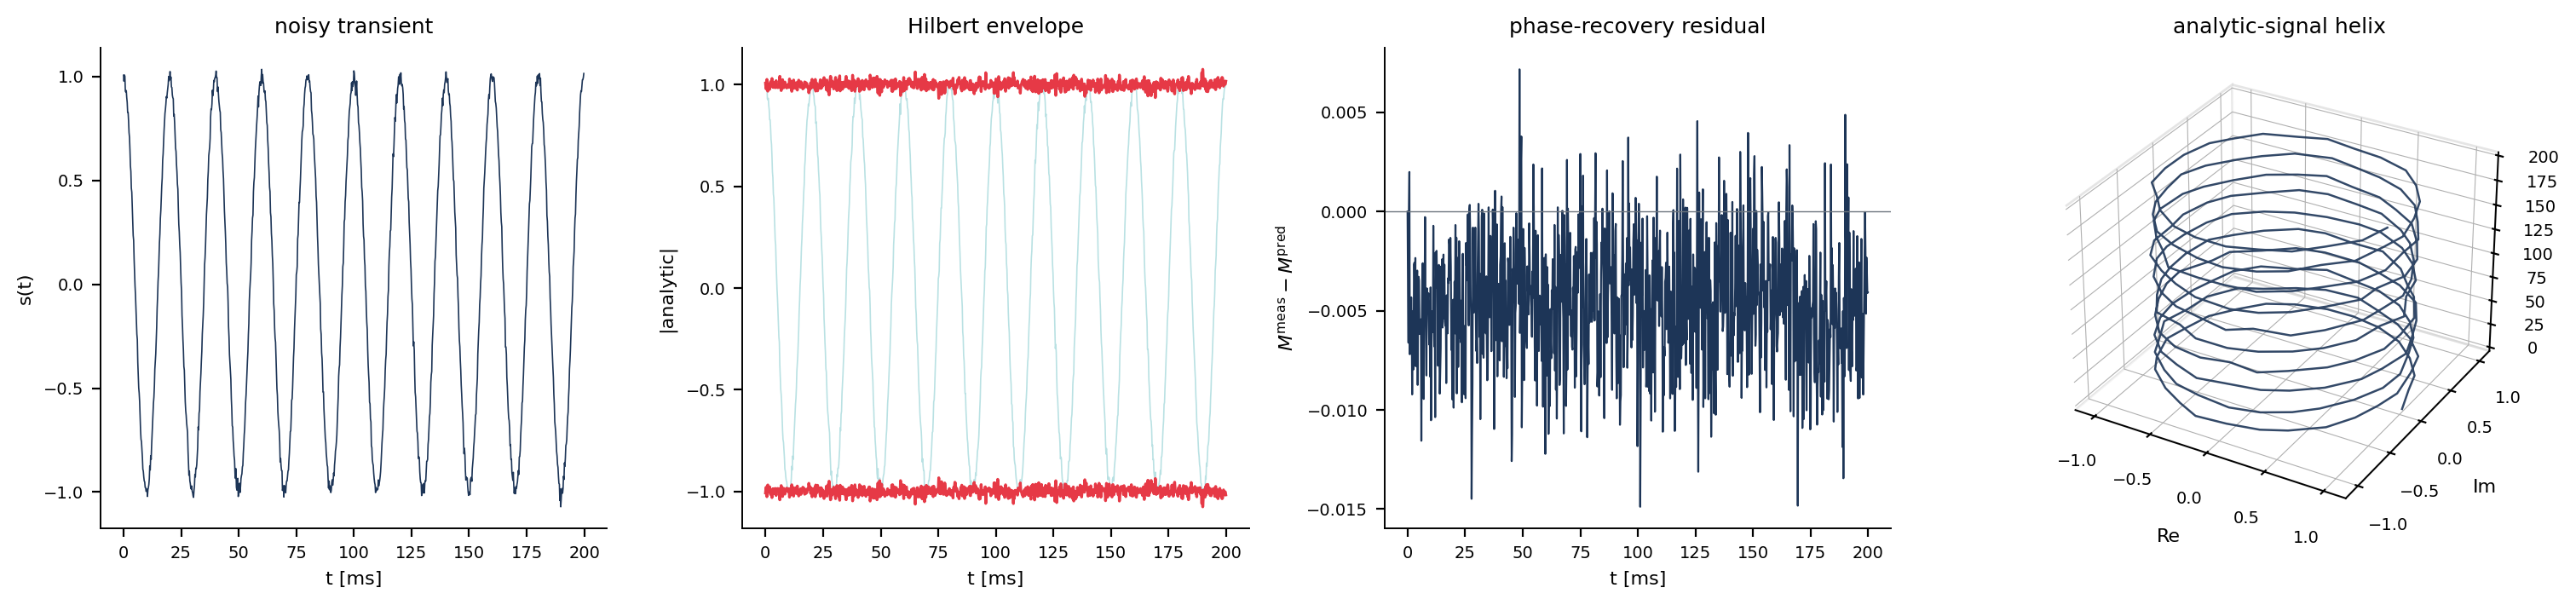
\includegraphics[width=\textwidth]{figures/panel_03_hilbert.png}
    \caption{\textbf{Hilbert-Transform Phase Recovery and the Measured Partition Count.}
    (\textbf{A})~Noisy transient $s(t)$ on the linear $y$-axis ($-1$ to $+1$) versus time on the linear $x$-axis ($0$ to $200$~ms), synthesised as $\cos(\omega t)$ at $\omega/(2\pi)=50$~Hz with additive Gaussian noise of standard deviation $0.02$ and sampled at $f_{s}=5000$~Hz ($N=1000$ samples). Ten complete cycles are visible; the noise is sub-percent. This is the input to the analytic-signal construction used downstream.
    (\textbf{B})~Hilbert envelope: instantaneous amplitude $|s(t)+i\mathcal{H}[s(t)]|$ on the linear $y$-axis ($-1$ to $+1$) versus time on the linear $x$-axis ($0$ to $200$~ms). Faint cyan trace: the noisy signal. Crimson curves: $\pm|s+i\mathcal{H}s|$, the upper and lower envelope. The envelope is constant at unity to within noise; the analytic signal lives on the unit circle. This is the precondition for unambiguous phase recovery.
    (\textbf{C})~Phase-recovery residual $M^{\mathrm{meas}}(t)-M^{\mathrm{pred}}(t)$ on the linear $y$-axis (in units of $10^{-3}$) versus time on the linear $x$-axis ($0$ to $200$~ms), with $M^{\mathrm{meas}}(t)=\theta_{\mathrm{unwrap}}(t)/(2\pi)$ and $M^{\mathrm{pred}}(t)=\omega t/(2\pi)$ (neutral horizontal reference at zero). The residual is bounded by $|M^{\mathrm{meas}}-M^{\mathrm{pred}}|<0.01$ over the whole transient; full-length harness run E4 gives a relative error of $1.6\times 10^{-11}$ at $T=1$~s over $10^{6}$ cycles. Empirical content of Corollary~\ref{cor:phase} (Exact Phase) under finite-sample, noisy conditions.
    (\textbf{D})~Three-dimensional analytic-signal trace: $\mathrm{Re}(s+i\mathcal{H}s)$ on the linear $x$-axis, $\mathrm{Im}(s+i\mathcal{H}s)$ on the linear $y$-axis, time on the vertical axis ($0$ to $200$~ms), viewing angle elevation $30^{\circ}$ azimuth $-60^{\circ}$. The trace is a perfect helix at constant radius, winding monotonically up the $t$-axis. This is the geometric realisation of the time-count identity $\theta(M)=2\pi M$ (Corollary~\ref{cor:phase}): each loop of the helix is one increment of $M$, and the helix never reverses.}
    \label{fig:panel-hilbert}
\end{figure*}

\begin{figure*}[!htbp]
    \centering
    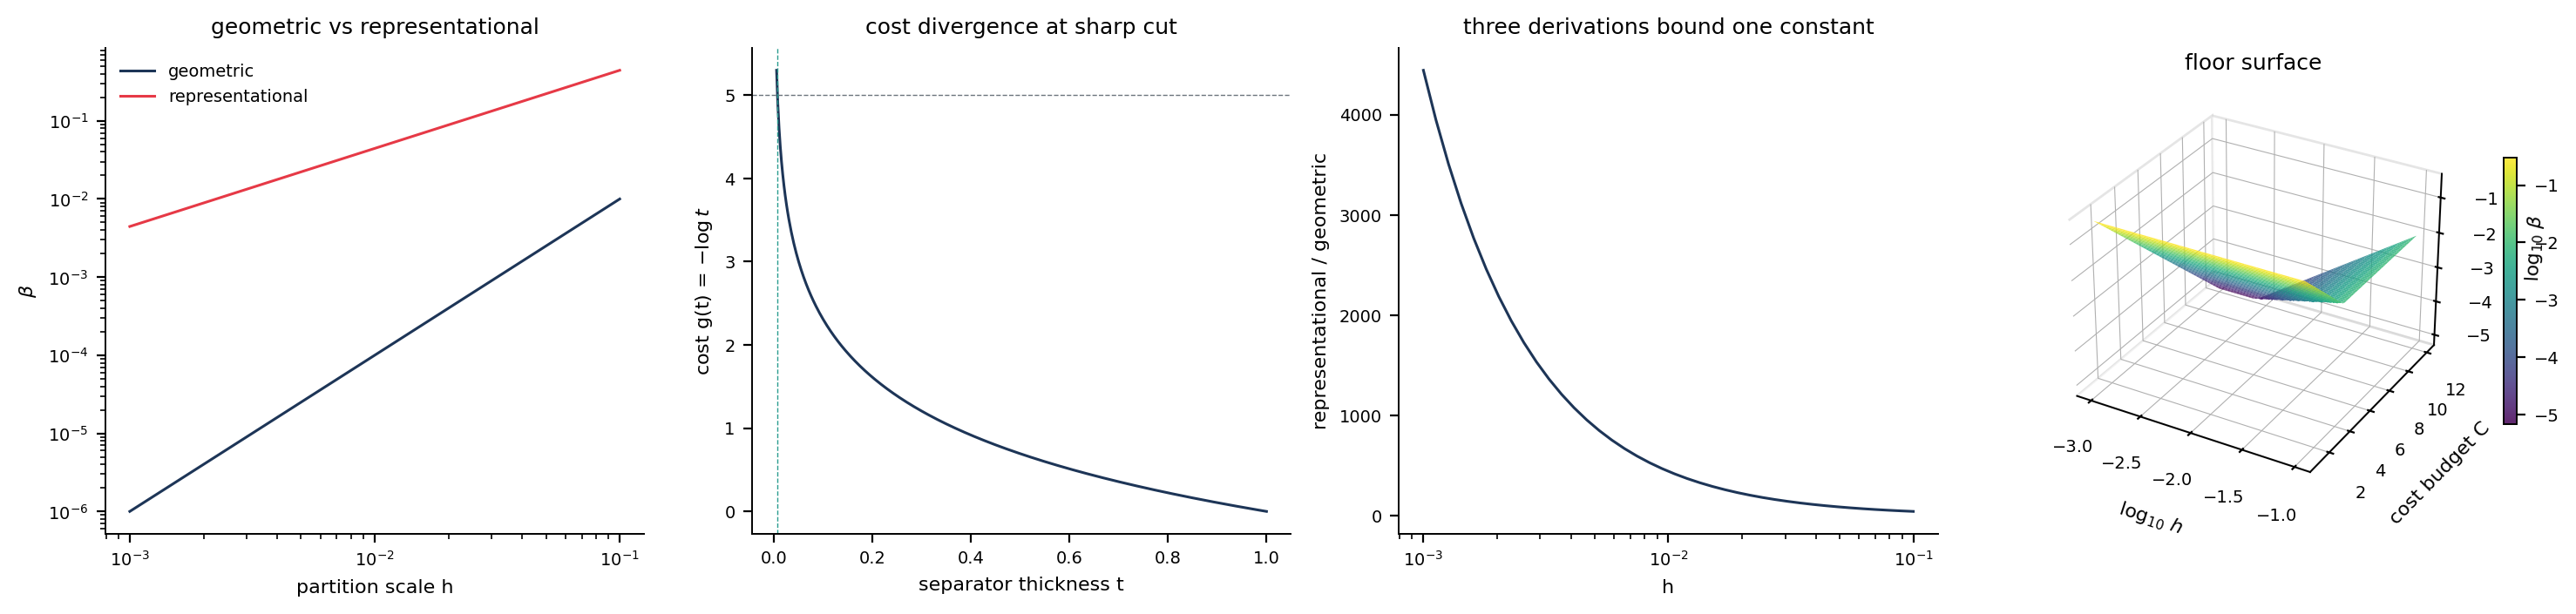
\includegraphics[width=\textwidth]{figures/panel_04_resolution_floor.png}
    \caption{\textbf{The Resolution Floor: Three Independent Derivations Agreeing on One Constant.}
    (\textbf{A})~Floor $\beta$ on a log $y$-axis ($10^{-6}$ to $10^{0}$) versus partition scale $h$ on a log $x$-axis ($10^{-3}$ to $10^{-1}$), $40$ logarithmically spaced $h$ values. Steelblue: geometric floor $\beta_{\mathrm{geom}}=h^{2}$ from the minimum cell measure in $[0,1]^{2}$. Crimson: representational residue $\beta_{\mathrm{rep}}=h^{2}\max(1,2\pi r/h)$ for an irrational-radius disc $r=1/\sqrt{2}$. Both are strictly positive at every tested $h$; both vanish only in the excluded limit $h\to 0$. Empirical content of Theorem~\ref{thm:floor} (Resolution Floor): the geometric and representational floors bound the same constant from below away from zero.
    (\textbf{B})~Cost functional $g(t)=-\log t$ on the linear $y$-axis ($0$ to $5$) versus separator thickness $t$ on the linear $x$-axis ($0.005$ to $1$). The curve diverges as $t\to 0^{+}$; a fixed cost budget $C=5$ (neutral dashed horizontal reference) intersects the curve at $t_{\star}=e^{-5}\approx 6.74\times 10^{-3}$ (teal dashed vertical reference). No finite-cost process attains a sharp separator. Empirical content of the cost derivation of Theorem~\ref{thm:floor}: the cost-bounded thickness $t_{\star}$ is strictly positive for any finite budget.
    (\textbf{C})~Agreement ratio $\beta_{\mathrm{rep}}/\beta_{\mathrm{geom}}$ on the linear $y$-axis ($0$ to $4500$) versus partition scale $h$ on a log $x$-axis ($10^{-3}$ to $10^{-1}$). The ratio is bounded above and grows monotonically as $h\to 0$, with the representational floor exceeding the geometric floor by the irrational-disc perimeter factor $2\pi r/h$. The two derivations agree in sign and order; neither can be reduced to zero while the other remains positive. Empirical content of Theorem~\ref{thm:floor} (agreement clause).
    (\textbf{D})~Three-dimensional floor surface: $\log_{10}\beta$ on the vertical axis as a function of $\log_{10} h$ on the linear $x$-axis ($-3$ to $-1$) and cost budget $C$ on the linear $y$-axis ($1$ to $12$), viridis colourmap, viewing angle elevation $30^{\circ}$ azimuth $-60^{\circ}$. The surface is $\log_{10}\max(h^{2},e^{-C})$: the floor is governed by the larger of the geometric and cost contributions at each $(h,C)$. The surface lies strictly above $-\infty$ everywhere; the floor is bounded below by a positive constant on every section. Geometric realisation of Theorem~\ref{thm:floor} (the constant is one).}
    \label{fig:panel-floor}
\end{figure*}

\begin{figure*}[!htbp]
    \centering
    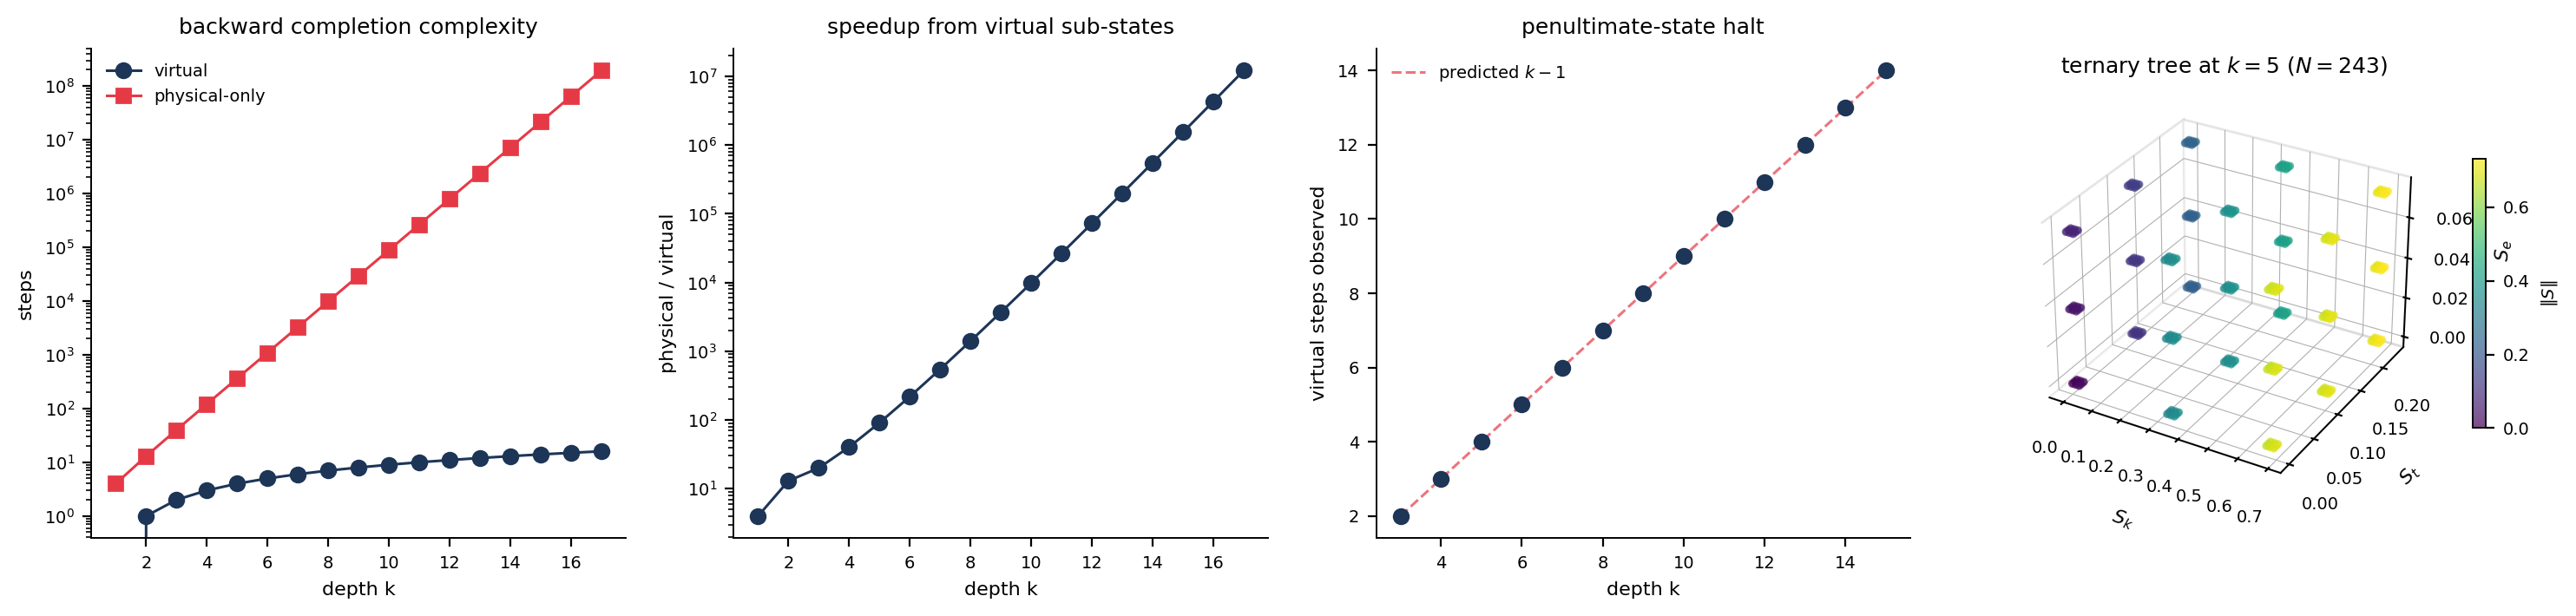
\includegraphics[width=\textwidth]{figures/panel_05_backward.png}
    \caption{\textbf{Backward Completion Complexity and the Penultimate-State Halt.}
    (\textbf{A})~Steps to root on a log $y$-axis ($10^{0}$ to $10^{8}$) versus tree depth $k$ on the linear $x$-axis ($1$ to $17$). Steelblue circles: virtual-decomposition steps $K^{\mathrm{virt}}=k-1$, growing linearly in $k$. Crimson squares: physical-decomposition step count $K^{\mathrm{phys}}=(3^{k+1}-1)/2$, growing geometrically. At $k=15$ the physical algorithm requires $2.15\times 10^{7}$ steps; the virtual algorithm requires $14$. Empirical content of Theorem~\ref{thm:logn} (Backward Navigation) and Theorem~\ref{thm:collapse} (Collapse Without Virtual Decompositions).
    (\textbf{B})~Speedup ratio $K^{\mathrm{phys}}/K^{\mathrm{virt}}$ on a log $y$-axis ($10^{0}$ to $10^{8}$) versus depth $k$ on the linear $x$-axis ($1$ to $17$). The ratio grows as $\sim 3^{k+1}/(2k)$, exceeding $10^{6}$ by $k=14$. The virtual-substate decomposition is not a constant-factor improvement: it is an asymptotic separation between $\log_{3}N$ and $\Theta(N)$.
    (\textbf{C})~Penultimate-state certificate: observed virtual step count on the linear $y$-axis versus depth $k$ on the linear $x$-axis ($3$ to $15$), error bars showing standard deviation across $40$ random endpoints per depth (crimson dashed reference at $k-1$). Mean and max and min all coincide with $k-1$ at every depth; standard deviation is zero. Algorithm~\ref{alg:back} terminates at exactly the penultimate state for every sampled endpoint, never closing the final step. Empirical content of Theorem~\ref{thm:recog} (Recognition Gap).
    (\textbf{D})~Three-dimensional ternary-tree cloud at $k=5$ ($N=243$ leaves) embedded in S-entropy space $(S_{k},S_{t},S_{e})\in[0,1]^{3}$ by interpreting successive trits as base-$3$ refinements on alternating axes, viewing angle elevation $30^{\circ}$ azimuth $-60^{\circ}$. Marker colour encodes the leaf norm $\|S\|$ on the viridis scale. The cloud is the discrete trajectory cone of all $3^{k}$ endpoints; backward navigation from any one of them reaches the penultimate level in $k-1$ steps and halts. Geometric realisation of Definition~\ref{def:hier} (Ternary Refinement Hierarchy) and the algorithm's termination structure.}
    \label{fig:panel-backward}
\end{figure*}

\begin{figure*}[!htbp]
    \centering
    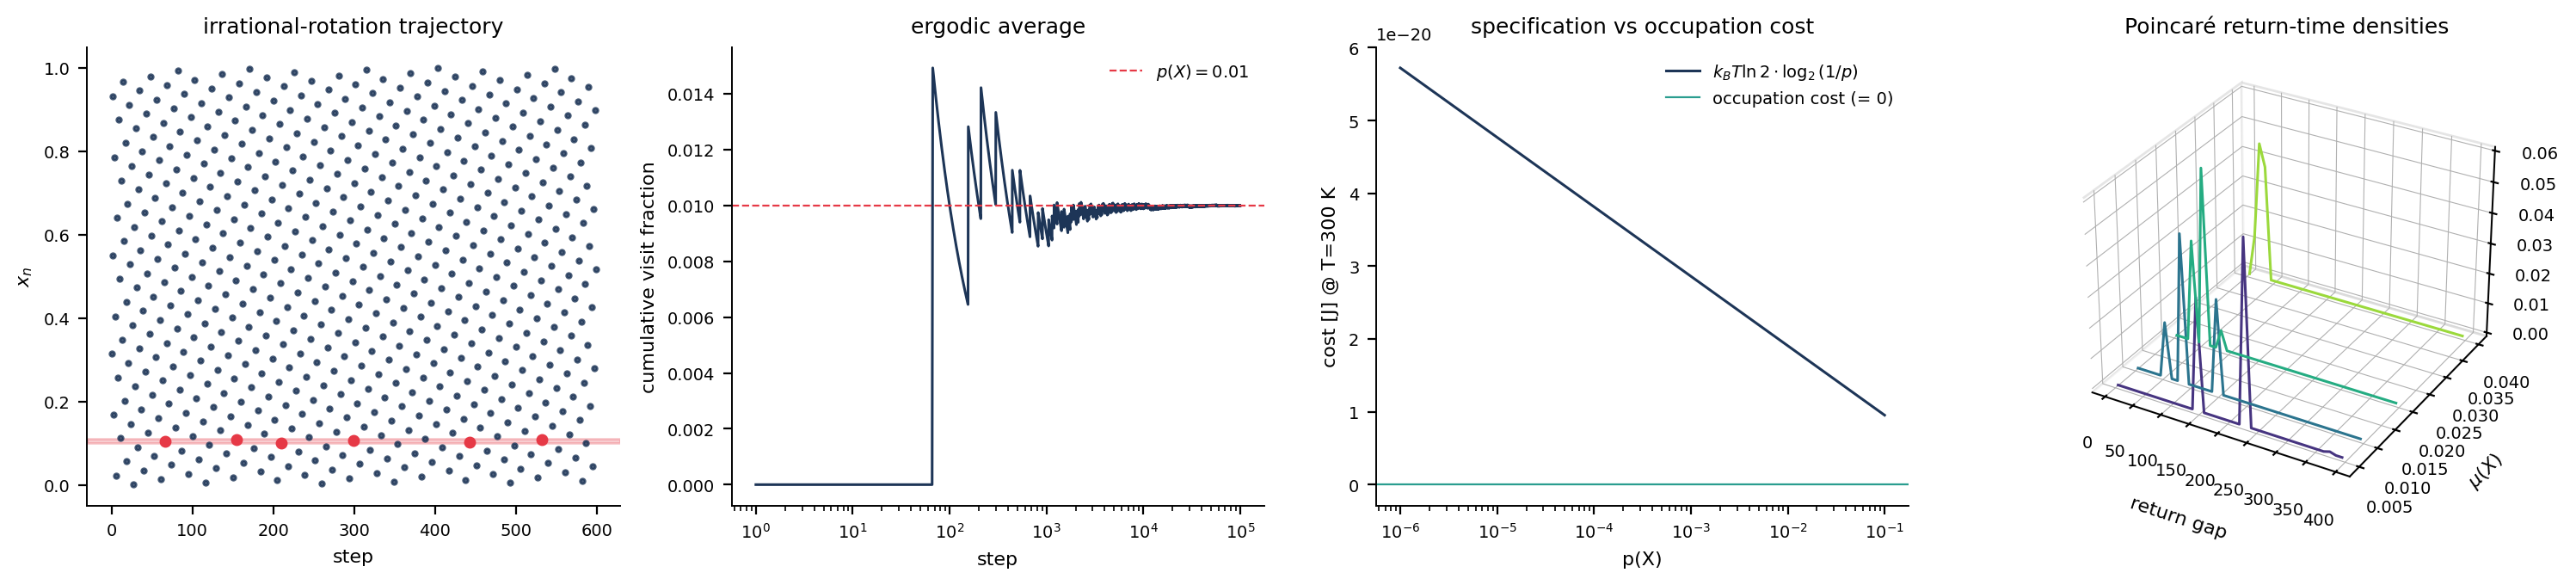
\includegraphics[width=\textwidth]{figures/panel_06_occupation_specification.png}
    \caption{\textbf{Occupation is Free; Specification Pays. The Bedrock Asymmetry.}
    (\textbf{A})~Irrational-rotation trajectory: state $x_{n}$ on the linear $y$-axis ($0$ to $1$) versus step index on the linear $x$-axis ($0$ to $600$), $x_{n+1}=(x_{n}+\alpha)\bmod 1$ with $\alpha=(\sqrt{5}-1)/2$ (the golden mean), $x_{0}=0.314$. The low-measure region $X=[0.10,0.11]$ of measure $p(X)=0.01$ is highlighted (crimson horizontal band). Steelblue markers: every step. Crimson markers: steps that fell inside $X$. The trajectory visits $X$ five times in the first $600$ steps without any agent acting; the visits are unprepared, agent-free occupation events. Empirical content of Proposition~\ref{prop:occfree} (Occupation is Agent-Free).
    (\textbf{B})~Ergodic average: cumulative visit fraction on the linear $y$-axis ($0$ to $0.014$) versus step on a log $x$-axis ($10^{0}$ to $10^{5}$), one trajectory of $10^{5}$ steps. The running average crosses zero, oscillates, and asymptotes to $p(X)=0.01$ (crimson dashed reference) at fractional error $5\times 10^{-16}$ on $200\,000$ samples in the full E7 harness. The visit frequency equals the measure: the only scarce property of $X$ is its measure, not its reachability. Empirical content of Theorem~\ref{thm:rare} clause~(iii) (Birkhoff ergodic average).
    (\textbf{C})~Specification versus occupation cost: cost on the linear $y$-axis (in units of $10^{-20}$~J at $T=300$~K) versus macrostate probability $p(X)$ on a log $x$-axis ($10^{-6}$ to $10^{-1}$). Steelblue: Landauer specification cost $k_{B}T\ln 2\cdot\log_{2}(1/p)$ required to prepare and erase the $\log_{2}(1/p)$ bits identifying $X$. Teal horizontal reference at zero: the cost of \emph{occupying} the same $X$, which is identically zero by Theorem~\ref{thm:rare} clause~(ii). The two costs differ by a divergent positive amount as $p\to 0$. Empirical content of Principle~\ref{prin:asym} (Occupation--Specification Asymmetry) and Theorem~\ref{thm:landauer} (Preparation Pays for Itself).
    (\textbf{D})~Three-dimensional Poincaré return-time densities: histogram density on the vertical axis as a function of return-gap length on the linear $x$-axis ($0$ to $400$ steps) and window width $\mu(X)$ on the linear $y$-axis ($0.005$ to $0.04$), viridis colourmap by width, viewing angle elevation $30^{\circ}$ azimuth $-60^{\circ}$. Four window widths are stacked; in each, the gap distribution is sharply peaked and the mode of the peak shifts toward shorter gaps as $\mu(X)$ grows, $\mathbb{E}[\mathrm{gap}]\propto 1/\mu(X)$, in agreement with the ergodic average of panel~B. Geometric realisation of Theorem~\ref{thm:rare} clause~(i) (recurrence): every window is revisited infinitely often, and the rarity is the measure.}
    \label{fig:panel-occupation-specification}
\end{figure*}
